\newcommand{\DeinName}{Pascal Fischer}
\newcommand{\MatrNo}{371778}
\newcommand{\TitelArbeit}{Entwicklung einer verschlüsselten Chat-basierten Plattform auf Basis des Matrix.org-Protokolls im Kontext von digitaler Gesundheit und Telemedizin}
\newcommand{\Fachgebiet}{Regelungssysteme}
\newcommand{\PrueferEins}{Dr.-Ing Thomas Schauer}
\newcommand{\PrueferZwei}{Prof.-Dr.-Ing. Clemens Gühmann}
\newcommand{\fachbereich}{Elektrotechnik und Informatik}

% entweder ein Datum h?ndisch eintragen, oder den Befehl \today nutzen
\newcommand{\Datum}{\today}

\makeglossary


%
% Einbinden des Headers, hier k?nnen auch weitere Einstellungen vorgenommen werden.
%%%%%%%%%%%%%%%%%%%%%%%%%%%%%%%%%%%%%%%%%%%%%%%%%%%%%%%
%																					%
%	In dieser Datei werden alle Packages eingebunden, 	%
% welche f�r das Dokument n�tig sind. Desweiteren 		%
% werden die Dokumentinformationen gesetzt.						%
%																											%
%%%%%%%%%%%%%%%%%%%%%%%%%%%%%%%%%%%%%%%%%%%%%%%%%%%%%%%
%
%	Die KOMAScript Dokumentklasse "scrbook" verwenden.
%
\documentclass[pdftex, 		%
							a4paper, 		% DIN A4 verwenden
							titlepage,	% separate Titelseite
							%draft,			%	Draft-Version, keine Bilder im pdf!
							final,			% Final-Version
							oneside,		% einseitiger Druck
							12pt,				% Schriftgr��e 12pt
							DIV=calc,
							%tocbasic,
							]{scrbook}	%	KOMAScript scrbook-Dokumentklasse

							\usepackage{geometry}
							\geometry{
								left=3cm,
								right=3cm,
								top=3cm,
								bottom=4cm,
								bindingoffset=5mm
							}

\usepackage{tikz}

%%%%%%%%%%%%%%%%%%%%%%%%%%%%%%%%%%%%%%%%%%%%%%%%%%%%%%%%
%	Einbinden der Pakete
%%%%%%%%%%%%%%%%%%%%%%%%%%%%%%%%%%%%%%%%%%%%%%%%%%%%%%%%

\usepackage[ngerman]{babel}

% PDF Dateien einbinden
\usepackage{pdfpages}

%Settings for PDF Pages to accept additonal versioned PDF files
\pdfminorversion=6
\pdfcompresslevel=9
\pdfobjcompresslevel=9

%Infos dazu unter: http://www.bakoma-tex.com/doc/latex/koma-script/scrhack.pdf
%Einige Pakete haben Probleme mit dem Komaskript.
\usepackage{scrhack}


% Definieren von eigenen benannten Farben.
% F�r sp�tere Verwendung in dem Dokument, definieren wir einzelne
% benannte Farben.
%
\usepackage{xcolor}
\definecolor{gray1}{gray}{0.92}
\definecolor{darkgreen}{rgb}{0,0.5,0}

\definecolor{urlLinkColor}{rgb}{0,0,0.5}
\definecolor{LinkColor}{rgb}{0,0,0}
\definecolor{ListingBackground}{rgb}{0.85,0.85,0.85}

\usepackage{pgf-umlsd}

\definecolor{delim}{RGB}{20,105,176}
\definecolor{numb}{RGB}{106, 109, 32}
\definecolor{string}{rgb}{0.64,0.08,0.08}
\rmfamily
\usepackage{amsfonts}
\usepackage[square,numbers]{natbib}
\usepackage{palatino}
\usepackage{amsmath}				% Schriftfamilie Palatino
%\usepackage[utf8]{inputenc}
%\usepackage[latin1]{inputenc} % Umlaute
\usepackage[utf8]{inputenc}
%\usepackage[dvips]{color}    	% f�r graue Boxen
%\usepackage[dvips]{graphicx} 	% Grafikpaket
\usepackage{multirow}
\usepackage{graphicx}
%\usepackage[table,xcdraw]{xcolor}
\usepackage{makeidx}   				% Paket zur Erzeugung eines Index
\usepackage{siunitx}
\sisetup{locale = DE}
\usepackage[normalem]{ulem}   % bietet Unterstreichungsvarianten
%\usepackage{picins} 					% Bilder im Absatz platzieren
\usepackage[T1]{fontenc}			% Erweiterten Zeichensatz aktivieren
\usepackage{multido}					% erm�glicht Schleifenartiges wiederholen von Befehlen
\usepackage{mdwlist}					% erm�glicht das Setzen des Z�hlers bei Aufz�hlungspunkten
\usepackage{paralist}					% Paket f�r Aufz�hlungen, erweitert Enumerate-Paket
\usepackage{longtable}				% mehrseitige Tabellen
\usepackage{tocbasic}
\parindent0pt           			% verzichte auf Einr�cken der ersten Zeile
\parskip1ex             			% Abstand zwischen den Abs�tzen

\usepackage{setspace}					% Paket zum Einstellen des Zeilenabstands
\onehalfspacing								% anderthalbfacher Zeilenabstand
%\doublespacing								% doppelter Zeilenabstand
%\singlespacing								% einfacher Zeilenabstand
\usepackage{float}
%\usepackage[german]{babel}
\usepackage[german=quotes]{csquotes} %Deutsche Anf�hrungszeichen
\usepackage{subfig}
\definecolor{LinkColor}{rgb}{0.1,0.1,0.1}
%\definecolor{ListingBackground}{rgb}{0.85,0.85,0.85}
\definecolor{ListingBackground}{rgb}{0.98,0.98,0.98}
\definecolor{gray}{rgb}{0.4,0.4,0.4}
\definecolor{darkblue}{rgb}{0.0,0.0,0.6}
\definecolor{cyan}{rgb}{0.0,0.6,0.6}



%
% Farbeinstellungen f�r die Links im PDF Dokument.
%
\makeindex

%-----------Paket f�r absolute Positionierung von Grafiken------------------
\usepackage[absolute]{textpos}
\setlength{\TPHorizModule}{1mm}
\setlength{\TPVertModule}{\TPHorizModule}

%-----------Aufz�hlungen und Einstellungen f�r Sourcecode-------------------
%\usepackage[savemem]{listings} %Bei wenig Arbeitsspeicher dies Option [savemem] aktivieren.
\usepackage{listings}
\lstloadlanguages{TeX,XML, Java} % TeX sprache laden, notwendig wegen option 'savemem'
\lstset{%
	language=[LaTeX]TeX,     % Sprache des Quellcodes ist TeX
	numbers=left,            % Zelennummern links
	stepnumber=1,            % Jede Zeile nummerieren.
	numbersep=5pt,           % 5pt Abstand zum Quellcode
	numberstyle=\tiny,       % Zeichengr�sse 'tiny' f�r die Nummern.
	breaklines=true,         % Zeilen umbrechen wenn notwendig.
	breakautoindent=true,    % Nach dem Zeilenumbruch Zeile einr�cken.
	postbreak=\space,        % Bei Leerzeichen umbrechen.
	tabsize=2,               % Tabulatorgr�sse 2
	basicstyle=\ttfamily\footnotesize, % Nichtproportionale Schrift, klein f�r den Quellcode
	showspaces=false,        % Leerzeichen nicht anzeigen.
	showstringspaces=false,  % Leerzeichen auch in Strings ('') nicht anzeigen.
	extendedchars=true,      % Alle Zeichen vom Latin1 Zeichensatz anzeigen.
	backgroundcolor=\color{ListingBackground}} % Hintergrundfarbe des Quellcodes setzen.


\lstset{
  basicstyle=\small\ttfamily,
  columns=fullflexible,
  showstringspaces=false,
  %commentstyle=\color{gray}\upshape
}
%neue Lang definieren, als Bsp.
\lstdefinelanguage{XML-changed}
{
  basicstyle=\footnotesize\ttfamily\bfseries,
  morestring=[b]",
  morestring=[s]{>}{<},
  morecomment=[s]{<?}{?>},
  stringstyle=\color{black},
  identifierstyle=\color{darkblue},
  keywordstyle=\color{cyan},
  morekeywords={xmlns,version,type}% list your attributes here
}

%-----------Caption Package-------------------
\usepackage{caption}
\DeclareCaptionFont{white}{\color{white}}
\DeclareCaptionFormat{listing}{\colorbox[cmyk]{0.43, 0.35, 0.35,0.01}{\parbox{\textwidth}{\hspace{15pt}#1#2#3}}}

\DeclareCaptionFormat{graphics}{\colorbox[cmyk]{0.43, 0.35, 0.35,0.01}{\parbox{\textwidth}{\hspace{15pt}#1#2#3}}}


\captionsetup[lstlisting]{format=listing,labelfont=white,textfont=white, singlelinecheck=false, margin=0pt, font={footnotesize}}

%-----------Header+Footer---------------------------------------------------
\usepackage{fancyhdr}					%
\pagestyle{fancy}							%

\fancyhead{}
\fancyfoot{}
\renewcommand{\headrulewidth}{0.4pt} % Kopzeilenlinie
\renewcommand{\footrulewidth}{0.0pt} % Fusszeilenlinie 0.0pt blendet sie aus

\renewcommand{\chaptermark}[1]{\markboth{\thechapter\quad#1}{}}
\renewcommand{\sectionmark}[1]{\markright{\thesection\quad#1}}

%\fancyhead[LO]{\small\sffamily\rightmark}
\fancyhead[LE,RO]{\slshape \rightmark}
\fancyhead[LO,RE]{\slshape \leftmark}
%\fancyhead[RO]{\small\sffamily\thepage}
\fancyfoot[C]{\thepage}

%-----------Um die Eidesstattliche Erkl�rung als PDF einzubinden-----------------------------------
%\usepackage{pdfpages}

%------------Glossar--------------------------------------------------------------
\usepackage{expdlist}
\usepackage{/home/pfischer/Uni/Bachelorarbeit/Bachelorarbeit/paper/src/glossar}

\renewcommand{\glshead}{\chapter*{Glossar}}
\renewcommand{\glentry}[2]{\glossary{#1@[#1] #2|glspage}}
\renewcommand{\glsgroup}[1]{{\listpart{\makebox[0pt][l]{\rule[-2pt]{\textwidth}{0.5pt}}{\textbf{\large #1}}}}}

\makeglossary

%Glossar mit Bordmitteln ------------------------------------------------------------------
%Darstellung des Glossars einstellen
%\usepackage[style=super, header=none, border=none, number=none, cols=2, toc=true]{glossary}
%\renewcommand{\glossaryname}{Glossar}
%\printglossary

% --- diverse Schriften -------------------------------------------------------------------
%\newcommand{\url}[1]{{\sf\small #1}}     % Hyperlinks


% -------F�r ToDo-Notes--------------------------------------------------------------------
\usepackage[color=red, shadow]{todonotes} % ", disable" deaktiviert ToDo-Notes
%Vereinfachtes "Inline-Todo"
\newcommand{\td}[1]{{\todo[inline]{#1}}}
\newcommand{\tdu}[1]{{\todo[inline, color=green!40]{#1}}}

\newcommand{\SubItem}[1]{
	{\setlength\itemindent{15pt} \item[-] #1}
}
\newcommand{\citepnum}[1]{[\citenum{#1}]}

%--------F�r Links-------------------------------------------------------------------------




%--------HyperRef konfigurieren-------------------------------------------------------------------------

\usepackage[
	pdftitle={\TitelArbeit},
	pdfauthor={\DeinName},
	pdfsubject={\TitelArbeit},
	pdfcreator={MiKTeX, LaTeX with hyperref and KOMA-Script auf Basis der Vorlage von seiler.it},
	pdfkeywords={Abschlussarbeit, TU Berlin, Universität},%weitere Keywords hier einf�gen
	pdfpagemode=UseOutlines,%
	pdfdisplaydoctitle=true,%
	pdflang=de%
]{hyperref}

\hypersetup{%
	colorlinks=true,%        Aktivieren von farbigen Links im Dokument (keine Rahmen)
	linkcolor=LinkColor,%    Farbe festlegen.
	citecolor=LinkColor,%    Farbe festlegen.
	filecolor=LinkColor,%    Farbe festlegen.
	menucolor=LinkColor,%    Farbe festlegen.
	urlcolor=LinkColor,%     Farbe von URL's im Dokument.
	bookmarksnumbered=true%  �berschriftsnummerierung im PDF Inhalt anzeigen.
}

\newcommand{\improvement}{\todo[inline, color=green]}
\newcommand{\change}{\todo[inline, color=blue]}
\newcommand{\unsure}{\todo[inline, color=violet]}
\newcommand{\eunorm}[1]{\lVert #1 \rVert_{\num{2}}}
\newcommand{\anfzch}[1]{\glqq #1\grqq{}}


\usepackage{enumitem}

\usepackage{tabularray}
% --------- Generates Chapter header ------------------------

\DeclareMathAlphabet\EuRoman{U}{eur}{m}{n}
\SetMathAlphabet\EuRoman{bold}{U}{eur}{b}{n}
\newcommand{\eurom}{\EuRoman}
\definecolor{nicered}{rgb}{.647,.129,.149}
\usepackage{etoolbox}

\makeatletter
\newsavebox{\feline@chapter}
\newcommand\feline@chapter@marker[1][4cm]{%
	\sbox\feline@chapter{%
		\resizebox{!}{#1}{\setlength{\fboxsep}{0pt}%
		\colorbox{white}{\color{black}$\eurom\thechapter$}}}%
	\raisebox{\depth}{\usebox{\feline@chapter}}%
}
\renewcommand*{\chapterformat}{%
	\sbox\feline@chapter{\feline@chapter@marker[1.61cm]}%
	\makebox[0pt][l]{%
		\makebox[\dimexpr\textwidth][r]{%
			\usebox\feline@chapter}}%
}
\makeatother

\preto\chapterheadendvskip{%
	\vspace*{-\parskip}%
	{\noindent\setlength\parfillskip{0pt plus 1fil}\rule{\textwidth}{.4pt}\par}%
}


\graphicspath{ {./source/images/pictures/} }

\lstdefinelanguage{json}{
    numbers=left,
    numberstyle=\small,
    frame=single,
    rulecolor=\color{black},
    showspaces=false,
    showtabs=false,
    breaklines=true,
    postbreak=\raisebox{0ex}[0ex][0ex]{\ensuremath{\color{gray}\hookrightarrow\space}},
    breakatwhitespace=true,
    basicstyle=\ttfamily\small,
    upquote=true,
    morestring=[b]",
    stringstyle=\color{string},
    literate=
    *{0}{{{\color{numb}0}}}{1}
        {1}{{{\color{numb}1}}}{1}
        {2}{{{\color{numb}2}}}{1}
        {3}{{{\color{numb}3}}}{1}
        {4}{{{\color{numb}4}}}{1}
        {5}{{{\color{numb}5}}}{1}
        {6}{{{\color{numb}6}}}{1}
        {7}{{{\color{numb}7}}}{1}
        {8}{{{\color{numb}8}}}{1}
        {9}{{{\color{numb}9}}}{1}
        {\{}{{{\color{delim}{\{}}}}{1}
        {\}}{{{\color{delim}{\}}}}}{1}
        {[}{{{\color{delim}{[}}}}{1}
        {]}{{{\color{delim}{]}}}}{1},
}


\newcommand\YAMLcolonstyle{\color{red}\mdseries}
\newcommand\YAMLkeystyle{\color{black}\bfseries}
\newcommand\YAMLvaluestyle{\color{blue}\mdseries}

\makeatletter

% here is a macro expanding to the name of the language
% (handy if you decide to change it further down the road)
\newcommand\language@yaml{yaml}

\expandafter\expandafter\expandafter\lstdefinelanguage
\expandafter{\language@yaml}
{
    keywords={true,false,null,y,n},
    keywordstyle=\color{darkgray}\bfseries,
    basicstyle=\YAMLkeystyle,                                 % assuming a key comes first
    sensitive=false,
    comment=[l]{\#},
    morecomment=[s]{/*}{*/},
    commentstyle=\color{purple}\ttfamily,
    stringstyle=\YAMLvaluestyle\ttfamily,
    moredelim=[l][\color{orange}]{\&},
    moredelim=[l][\color{magenta}]{*},
    moredelim=**[il][\YAMLcolonstyle{:}\YAMLvaluestyle]{:},   % switch to value style at :
    morestring=[b]',
    morestring=[b]",
    literate =    {---}{{\ProcessThreeDashes}}3
        {>}{{\textcolor{red}\textgreater}}1
        {|}{{\textcolor{red}\textbar}}1
        {\ -\ }{{\mdseries\ -\ }}3,
}

% switch to key style at EOL
\lst@AddToHook{EveryLine}{\ifx\lst@language\language@yaml\YAMLkeystyle\fi}
\makeatother

\newcommand\ProcessThreeDashes{\llap{\color{cyan}\mdseries-{-}-}}


% Beginn des Dokuments
\begin{document}

%Zitiert alle Referenzen, ohne Sie hier zu listen. Dadurch erscheinen alle Quellen im %Literaturverzeichnis, auch wenn sie im Text nicht genutzt werden.
%Bitte nur f?r Testzwecke verwenden.
    \nocite{*}


% Einbinden des Deckblatts

    \frontmatter
    % erste Seite (Titelseite) der Diplomarbeit mit Titel, Name usw...

\newsavebox{\Prof}
\savebox{\Prof}{Erster Prüfer }

\newsavebox{\Betr}
\savebox{\Betr}{Zweiter Prüfer }
\begin{titlepage}

%\begin{minipage}[h]{0.5\textwidth}
%		\raggedright
%		\includegraphics[height=4cm]{source/images/Logo/TU-Berlin-Logo.png}
%	\end{minipage}
%	\begin{minipage}[h]{0.5\textwidth}
%		\raggedleft
%		\includegraphics[height=5cm]{source/images/Logo/sensorstim_logo.png}
%	\end{minipage}


	\begin{figure}
		\begin{center}
			
\includegraphics[height=4cm]{source/images/Logo/TU_Berlin_Logo.png}
		\end{center}
	\end{figure}

	\begin{center}
%\includegraphics[height=2cm]{source/images/logo_mirolab.png}

	{\Large Technische Universität Berlin}\\[1mm]
	{\large Fakultät Elektrotechnik und Informatik}\\
	{\large Fachgebiet \Fachgebiet}\\
	\vspace{1cm}
	{\LARGE  Bachelorarbeit}

	\vspace{0.5cm}

	{\LARGE\textbf{ \TitelArbeit}}\\


	\vspace{1.cm}

	von\\[2mm]

	\textbf{\large{\DeinName}}\\
%\vspace{1.5cm}
	Matrikelnummer: \MatrNo\\[1cm]

	Betreuer: Ardit Dvorani\\[2mm]

	\usebox{\Prof: \PrueferEins} \\
	\usebox{\Betr: \PrueferZwei} \\

	\vspace{1cm}
	Berlin, \today
	\end{center}
\end{titlepage}
    \hypersetup{pageanchor=false}

    \newpage
    \section*{Zusammenfassung}
    In dieser Arbeit befasst sich mit ....

    \section*{Abstract}\label{sec:abstract}
    This paper describes how to ...
    \newpage
    \chapter*{Eidesstattliche Erklärung}\label{ch:eidesstattliche-erklarung}
    Hiermit erkläre ich, dass ich die vorliegende Arbeit selbstständig und eigenhändig sowie ohne
    unerlaubte fremde Hilfe und ausschließlich unter Verwendung der aufgeführten Quellen und
    Hilfsmittel angefertigt habe.\\
    \vspace{1cm}\\
    Berlin, den \underline{\hspace{3cm}} \hfill \DeinName \underline{\hspace{4cm}}

    \newpage
    \tableofcontents

    \mainmatter

    \newpage
    \chapter{Einleitung}\label{ch:einleitung}

    \section{Motivation}\label{sec:motivation}
    Die Digitalisierung findet immer Einzug in unser alltägliches Leben, so auch in der Medizin.
    Der Einsatz neuer digitaler Innovationen soll eine bestmögliche Versorgung der Patienten gewährleisten.
    Eine große Herausforderung ist der demografische Wandel und der Mangel an Fachärztinnen und Fachärzten in ländlichen Regionen.
    Um dem entgegenzuwirken, wurde das Verbot von Fernbehandlungen nach der Musterberufsordnung der Ärzte (MBO-Ä) im Jahr 2018~\cite{beschlussprotokol} aufgehoben.
    Dies ermöglicht eine bequeme und schnelle Behandlung von zu Hause.
    So muss beispielsweise für eine Krankschreibung oder ein Folgerezept nicht extra eine Arztpraxis aufgesucht werden.
    Hierdurch können lange Anfahrtswege und Wartezeiten vermieden werden.
    Besonders seit Beginn der Coronapandemie im Jahr 2019 werden Rufe nach Softwarelösungen für den Einsatz in der Telemedizin immer lauter.
    Viele Bürger fürchten jedoch um die Sicherheit ihrer Daten, weshalb das Thema Datenschutz eine besondere Rolle beim Einsatz von Telemedizin spielt.
    Auch vonseiten des Gesetzgebers gelten strenge Vorgaben im Umgang mit personenbezogenen Daten, besonders wenn es sich hierbei um medizinische Daten handelt.
    Viele gängige Messenger wie WhatsApp oder Telegramm unterstützen zwar eine End-to-End-Verschlüsselung der gesendeten Nachrichten, jedoch entsprechen sie nicht den Datenschutz Vorschriften, die in der Datenschutz-Grundverordnung der Europäischen Union (DSGVO) festgelegt sind.
    Aus diesem Grund müssen Alternativen geschaffen werden, die für den Einsatz in der Telemedizin zugelassen sind.

    \newpage
    \section{Zielsetzung}\label{sec:zielsetzung}
    Ziel dieser Arbeit ist es eine Plattform zu entwickeln, welchen es Ärzten und Patienten ermöglicht in Kontakt zu treten und Nachrichten auszutauschen.
    Hierfür soll eine Chat-basierte Plattform auf Basis des Matrix.org-Protokolls entwickelt werden.
    Es muss eine App für die Nutzung der Plattform implementiert werden sowie die benötigte Infrastruktur bereitgestellt werden, um Nachrichten und Daten zu speichern und zu übermitteln.
    Die App ist in der Programmiersprache Swift zu implementieren und soll auf allen gängigen iOS Geräten unterstützt werden.
    Die Infrastruktur soll isoliert laufen und nicht an das existierende Matrix-Netzwerk angeschlossen werden.
    Da medizinische Daten dem Datenschutz in besonderer Maße unterliegen, ist es besonders wichtig,
    dass jegliche Art von Kommunikation zwischen Ärzten und Patienten stets verschlüsselt ist.
    Es muss gewährleistet sein, dass zu jedem Zeitpunkt alle personenbezogenen Daten vor dem Zugriff unerlaubter Dritter geschützt sind.
    Außerdem muss darauf geachtet werden, dass die Plattform keine der Vorschriften aus der DSGVO verletzt.

    \section{Aufbau der Arbeit}\label{sec:aufbau-der-arbeit}
    Zu Beginn werden die theoretischen Grundlagen, die für die Entwicklung der Plattform von Bedeutung sind, erläutert.
    Es werden die zur Implementierung der Plattform genutzten Technologien vorgestellt und deren Verwendung beschrieben.
    Danach werden einige ähnliche Projekte vorgestellt und analysiert.
    Basierend auf dieser Analyse werden eine Reihe von technischen Anforderungen definiert, welche von der implementierten Plattform erfüllt werden sollen.
    Anschließend wird die implementierte Plattform vorgestellt und deren Funktionsweise erklärt.
    Abschließend wird die Plattform unter Betrachtung der definierten Anforderungen evaluiert.

    \newpage
    \chapter{Theoretische Grundlagen}\label{ch:theoretische-grundlagen}
    In diesem Kapitel werden zunächst die theoretischen Grundlagen, welche die Implementierung der Plattform beeinflusst haben, vermittelt.
    Zuerst werden die gesetzlichen Ansprüche an eine Messaging-Plattform im medizinischen Bereich beleuchtet.
    Anschließend wird das Matrix-Protokoll vorgestellt und seine allgemeine Funktionsweise beschrieben.
    Außerdem werden die zur Verschlüsselung verwendeten Algorithmen erklärt und die dafür benötigten Schlüssel aufgezeigt.
    Es wird das REST Paradigma vorgestellt, welches die Grundlage für die Kommunikation zwischen Client und Server bildet.
    Des Weiteren wird die MVVM Architektur erläutern, welche bei der Implementierung der App verfolgt wurde.

    \section{Datenschutz im Gesundheitswesen}\label{sec:datenschutz-im-gesundheitswesen}
    Die rechtlichen Rahmenbedingungen für das Speichern und Verarbeiten medizinischer Daten sind in der EU-Datenschutz-Grundverordnung\footnote{https://dsgvo-gesetz.de/} (DSGVO) festgelegt.
    Diese fordert ebenfalls zur Einhaltung des IT-Sicherheitsgesetzes und des E-Health-Gesetzes auf.
    Medizinische Daten werden vom Gesetzgeber in besonderem Maße geschützt, da sie besonders sensible Informationen enthalten~\cite{datenschutzimgesundeitswesen}.

    \textit{Das am 29. Dezember 2015 in Kraft getretene "Gesetz für sichere digitale Kommunikation und Anwendungen im Gesundheitswesen (E-Health-Gesetz)" hat die ersten Weichen für den Aufbau der sicheren Telematikinfrastruktur (TI) und die Einführung medizinischer digitaler Anwendungen gestellt.
    Ziel dieses Gesetzes war es, die Chancen der Digitalisierung für die Gesundheitsversorgung zu nutzen und eine schnelle Einführung medizinischer Anwendungen für die Patientinnen und Patienten zu ermöglichen.}~\cite{ehealthgesetz}

    Ein Teil der Telematikinfrastruktur ist der TI-Messenger der Gematik GmbH, welcher im Abschnitt~\ref{subsec:ti-messenger} genauer betrachtet wird.\\
    Am 07.11.2019 hat die Konferenz der unabhängigen Datenschutzaufsichtsbehörden des Bundes und der Länder ein Whitepaper veröffentlicht, welche die \("\)Technischen Datenschutzanforderungen an Messenger-Dienste im\linebreak
    Krankenhausbereich\("\) aus Sicht der DSGVO~\cite{datenschutzkonferenz} offenlegt.
    Einige dieser Anforderungen sind:
    \begin{enumerate}[label={(\arabic*)}]
        \item Die Applikation muss über die Möglichkeit verfügen, die Nutzung bzw. den Zugriff
    auf die darüber gespeicherten Daten an eine eigene vorherige Authentifizierung (z.B.
    PIN, Fingerabdruck etc.) zu knüpfen.
        \item Die Applikation muss über die Möglichkeit verfügen, Kontaktdaten von
    Kommunikationsteilnehmern in einem eigenen, vom allgemeinen Adressbuch des
    Smartphones getrennten Speicher abzulegen.
        \item Sie muss weiterhin über die Möglichkeit verfügen,
    Nachrichten sowie Dateianhänge wie Bilder, Videos, Dokumente etc. ausschließlich
    in einem eigenen, von den allgemeinen Speicherbereichen des Smartphones
    getrennten Speicher in verschlüsselter Form abzulegen.
        \item Eine Kommunikation über die Messenger-Applikation sollte nur auf
    der Grundlage einer verlässlichen Identifizierung und Authentifizierung der
    Kommunikationspartner möglich sein.
        \item Werden elektronische Signaturen oder andere elektronischer Zertifikate genutzt,
    muss ein Zertifikatsmanagement vorhanden sein. Dies beinhaltet die Sicherstellung,
    dass elektronische Schlüssel oder Zertifikate eindeutig einer juristischen oder
    natürlichen Person zugeordnet werden, aber auch die Überprüfung der Gültigkeit der
    elektronischen Schlüssel bzw. Zertifikate. Insbesondere müssen kompromittierte
    Schlüsseln bzw. Zertifikate bzw. unbrauchbar gemacht werden können.
        \item Die Applikation muss über die Möglichkeit verfügen, die über sie verwalteten Daten
    gezielt oder allgemein zu löschen.
        \item Soweit die Speicherung unter Einhaltung von Art. 28 DS-GVO durch einen Dienstleister übernommen wird, welcher nicht die Anforderungen des Art. 9 Abs. 3 DS-GVO erfüllt,
    muss die Möglichkeit bestehen, die Daten nach dem Stand der Technik vor ihrer
    Übergabe derart zu verschlüsseln, dass eine Entschlüsselung nur mit einem
    Schlüssel möglich ist, der nicht an den Dienstleister offenbart und separat gesichert
    wird.
        \item Die Vertraulichkeit und Integrität der über den Messenger-Dienst geführten
    ärztlichen Kommunikation muss unter Berücksichtigung des Stands der Technik
    über eine Ende-zu-Ende-Verschlüsselung zwischen den
    Kommunikationsteilnehmern gewährleistet werden.
    \end{enumerate}


    \newpage
    \section{Matrix}\label{sec:matrix}

    \subsection{Matrix Protokoll}\label{subsec:matrix-protokoll}
    Das Matrix-Protokoll ist ein offener Standard für dezentrale Echtzeitkommunikation im Internet.
    Es ist ein Open-Source-Projekt, welches unter Aufsicht der Matrix.org Foundation, einer Non-Profit-Organisation aus England, entwickelt wird.
    Das Team besteht aus 12 Personen, viele von ihnen mit weitreichenden Erfahrungen im Bereich VoIP- und Messaging-Apps für Mobilgeräte.
    Die Entwicklung begann im Jahr 2014 und ist seit Juni 2019 für den Einsatz im Produktionsbetrieb geeignet~\cite{matrixfaq}.
    Mittlerweile gibt es zahlreiche Beiträge aus der Community, wodurch das Projekt weiter vorangetrieben wird.
    Das ursprüngliche Ziel des Projektes war es ein Protokoll zu entwickeln, welches es Usern ermöglichen soll, anderen Usern Nachrichten zu schreiben oder diese anzurufen, unabhängig davon welche Plattform diese benutzen.
    Langfristig soll Matrix ein generisches System zum Messaging und Datensynchronisation über HTTP für das ganze Internet bilden~\cite{matrixfaq}.
    Hierzu definiert Matrix eine Reihe von REST-APIs:
    \begin{description}[leftmargin=!,labelwidth=5.5cm]
        \item [Client-Server-API\footnotemark] \footnotetext{https://spec.matrix.org/v1.4/client-server-api/} zur Kommunikation zwischen Matrix kompatiblen Clients und einem Homeserver
        \item [Server-Server-API\footnotemark] \footnotetext{https://spec.matrix.org/v1.4/server-server-api/} zum Nachrichtenaustausch und Synchronisation zwischen mehreren Homservern
        \item [Application-Service-API\footnotemark] \footnotetext{https://spec.matrix.org/v1.4/application-service-api/} zur Erweiterung der Funktionalität von Matrix und Integration anderer Systeme
        \item [Identity-Service-API\footnotemark] \footnotetext{https://spec.matrix.org/v1.4/identity-service-api/} beschreibt das Mapping zwischen Drittanbietern
        \item [Push-Gateway-API\footnotemark] \footnotetext{https://spec.matrix.org/v1.4/push-gateway-api/} zum Versenden von Push Notifications an Clients bei eintreffen neuer Events auf dem Homeserver
    \end{description}

    \subsection{Funktionsweise}\label{subsec:funktionsweise}
    Matrix beschreibt sich selbst als dezentralen Konversationsspeicher\cite{matrix}.
    Hierbei werden alle Nachrichten (Events) die von einem User an einen Raum verschickt werden auf seinem Homeserver gespeichert.
    Ein Homeserver beschreibt einen Knoten im Matrix-Netzwerk.
    Jeder Client ist mit einem einzigen Homeserver verbunden.
    Damit eine Konversation stattfinden kann, sorgt der Homeserver dafür, dass die vom User gesendete Nachricht an die Homeserver der anderen Teilnehmer eines Raumes synchronisiert wird.
    Somit hält jeder Homeserver eine Kopie des vollständigen Konversationsverlaufs.
    Selbst wenn ein Server zwischenzeitlich ausfällt, können die anderen Teilnehmer ihre Konversation fortführen.
    Sollte der ausgefallene Server wieder aktiv werden, kann er die verpassten Nachrichten nachtragen~\cite{matrix}.
    Alle Nachrichten einer Konversation werden in einem Directed Acyclic Graph (DAG) gespeichert.
    Dieser wird im Kontext von Matrix als Event-Graph bezeichnet.
    Hierbei besitzt jedes Event einen oder mehrere Eltern (außer der Wurzelknoten).
    Somit lässt sich der Event-Graph chronologisch ordnen.
    Hierzu wird jedem Event ein ganzzahlig, positiver Wert \texttt{depth} zugewiesen, welcher die Reihenfolge der Events beschreibt~\cite{eventgraph}.\\
    In Abbildung~\ref{fig:matrixfunktionsweise} ist eine Beispielsituation für einen Raum zwischen Alice, Bob und Charlie gezeigt.
    Jeder der Teilnehmer ist mit seinem eigenen Homeserver verbunden.
    \begin{figure}[h]
        \centering
        

% Pattern Info

\tikzset{
    pattern size/.store in=\mcSize,
    pattern size = 5pt,
    pattern thickness/.store in=\mcThickness,
    pattern thickness = 0.3pt,
    pattern radius/.store in=\mcRadius,
    pattern radius = 1pt}
\makeatletter
\pgfutil@ifundefined{pgf@pattern@name@_2eflf89xd}{
    \pgfdeclarepatternformonly[\mcThickness,\mcSize]{_2eflf89xd}
        {\pgfqpoint{0pt}{0pt}}
        {\pgfpoint{\mcSize}{\mcSize}}
        {\pgfpoint{\mcSize}{\mcSize}}
        {
        \pgfsetcolor{\tikz@pattern@color}
        \pgfsetlinewidth{\mcThickness}
        \pgfpathmoveto{\pgfqpoint{0pt}{\mcSize}}
        \pgfpathlineto{\pgfpoint{\mcSize+\mcThickness}{-\mcThickness}}
        \pgfpathmoveto{\pgfqpoint{0pt}{0pt}}
        \pgfpathlineto{\pgfpoint{\mcSize+\mcThickness}{\mcSize+\mcThickness}}
        \pgfusepath{stroke}
    }}
\makeatother

% Pattern Info

\tikzset{
    pattern size/.store in=\mcSize,
    pattern size = 5pt,
    pattern thickness/.store in=\mcThickness,
    pattern thickness = 0.3pt,
    pattern radius/.store in=\mcRadius,
    pattern radius = 1pt}
\makeatletter
\pgfutil@ifundefined{pgf@pattern@name@_a6o28e1ro}{
    \pgfdeclarepatternformonly[\mcThickness,\mcSize]{_a6o28e1ro}
        {\pgfqpoint{0pt}{0pt}}
        {\pgfpoint{\mcSize+\mcThickness}{\mcSize+\mcThickness}}
        {\pgfpoint{\mcSize}{\mcSize}}
        {
        \pgfsetcolor{\tikz@pattern@color}
        \pgfsetlinewidth{\mcThickness}
        \pgfpathmoveto{\pgfqpoint{0pt}{0pt}}
        \pgfpathlineto{\pgfpoint{\mcSize+\mcThickness}{\mcSize+\mcThickness}}
        \pgfusepath{stroke}
    }}
\makeatother

% Pattern Info

\tikzset{
    pattern size/.store in=\mcSize,
    pattern size = 5pt,
    pattern thickness/.store in=\mcThickness,
    pattern thickness = 0.3pt,
    pattern radius/.store in=\mcRadius,
    pattern radius = 1pt}
\makeatletter
\pgfutil@ifundefined{pgf@pattern@name@_zxxkiapd2}{
    \makeatletter
    \pgfdeclarepatternformonly[\mcRadius,\mcThickness,\mcSize]{_zxxkiapd2}
        {\pgfpoint{-0.5*\mcSize}{-0.5*\mcSize}}
        {\pgfpoint{0.5*\mcSize}{0.5*\mcSize}}
        {\pgfpoint{\mcSize}{\mcSize}}
        {
        \pgfsetcolor{\tikz@pattern@color}
        \pgfsetlinewidth{\mcThickness}
        \pgfpathcircle\pgfpointorigin{\mcRadius}
        \pgfusepath{stroke}
    }}
\makeatother

% Pattern Info

\tikzset{
    pattern size/.store in=\mcSize,
    pattern size = 5pt,
    pattern thickness/.store in=\mcThickness,
    pattern thickness = 0.3pt,
    pattern radius/.store in=\mcRadius,
    pattern radius = 1pt}
\makeatletter
\pgfutil@ifundefined{pgf@pattern@name@_7ksk1ug9w}{
    \pgfdeclarepatternformonly[\mcThickness,\mcSize]{_7ksk1ug9w}
        {\pgfqpoint{0pt}{0pt}}
        {\pgfpoint{\mcSize}{\mcSize}}
        {\pgfpoint{\mcSize}{\mcSize}}
        {
        \pgfsetcolor{\tikz@pattern@color}
        \pgfsetlinewidth{\mcThickness}
        \pgfpathmoveto{\pgfqpoint{0pt}{\mcSize}}
        \pgfpathlineto{\pgfpoint{\mcSize+\mcThickness}{-\mcThickness}}
        \pgfpathmoveto{\pgfqpoint{0pt}{0pt}}
        \pgfpathlineto{\pgfpoint{\mcSize+\mcThickness}{\mcSize+\mcThickness}}
        \pgfusepath{stroke}
    }}
\makeatother

% Pattern Info

\tikzset{
    pattern size/.store in=\mcSize,
    pattern size = 5pt,
    pattern thickness/.store in=\mcThickness,
    pattern thickness = 0.3pt,
    pattern radius/.store in=\mcRadius,
    pattern radius = 1pt}
\makeatletter
\pgfutil@ifundefined{pgf@pattern@name@_qh7wu9oqq}{
    \pgfdeclarepatternformonly[\mcThickness,\mcSize]{_qh7wu9oqq}
        {\pgfqpoint{0pt}{0pt}}
        {\pgfpoint{\mcSize+\mcThickness}{\mcSize+\mcThickness}}
        {\pgfpoint{\mcSize}{\mcSize}}
        {
        \pgfsetcolor{\tikz@pattern@color}
        \pgfsetlinewidth{\mcThickness}
        \pgfpathmoveto{\pgfqpoint{0pt}{0pt}}
        \pgfpathlineto{\pgfpoint{\mcSize+\mcThickness}{\mcSize+\mcThickness}}
        \pgfusepath{stroke}
    }}
\makeatother

% Pattern Info

\tikzset{
    pattern size/.store in=\mcSize,
    pattern size = 5pt,
    pattern thickness/.store in=\mcThickness,
    pattern thickness = 0.3pt,
    pattern radius/.store in=\mcRadius,
    pattern radius = 1pt}
\makeatletter
\pgfutil@ifundefined{pgf@pattern@name@_2e10vbjsb}{
    \makeatletter
    \pgfdeclarepatternformonly[\mcRadius,\mcThickness,\mcSize]{_2e10vbjsb}
        {\pgfpoint{-0.5*\mcSize}{-0.5*\mcSize}}
        {\pgfpoint{0.5*\mcSize}{0.5*\mcSize}}
        {\pgfpoint{\mcSize}{\mcSize}}
        {
        \pgfsetcolor{\tikz@pattern@color}
        \pgfsetlinewidth{\mcThickness}
        \pgfpathcircle\pgfpointorigin{\mcRadius}
        \pgfusepath{stroke}
    }}
\makeatother
\tikzset{every picture/.style={line width=0.75pt}} %set default line width to 0.75pt

\begin{tikzpicture}[x=0.75pt,y=0.75pt,yscale=-1,xscale=1]
%uncomment if require: \path (0,580); %set diagram left start at 0, and has height of 580

%Shape: Ellipse [id:dp9373687458561233]
    \draw  [pattern=_2eflf89xd,pattern size=6pt,pattern thickness=0.75pt,pattern radius=0pt, pattern color={rgb, 255:red, 0; green, 0; blue, 0}] (246.86,261.57) .. controls (246.86,241.87) and (262.73,225.89) .. (282.31,225.89) .. controls (301.89,225.89) and (317.76,241.87) .. (317.76,261.57) .. controls (317.76,281.28) and (301.89,297.25) .. (282.31,297.25) .. controls (262.73,297.25) and (246.86,281.28) .. (246.86,261.57) -- cycle ;
%Shape: Ellipse [id:dp21917683521442988]
    \draw  [pattern=_a6o28e1ro,pattern size=6pt,pattern thickness=0.75pt,pattern radius=0pt, pattern color={rgb, 255:red, 0; green, 0; blue, 0}] (362.46,194.09) .. controls (362.46,174.39) and (378.33,158.41) .. (397.91,158.41) .. controls (417.49,158.41) and (433.36,174.39) .. (433.36,194.09) .. controls (433.36,213.8) and (417.49,229.77) .. (397.91,229.77) .. controls (378.33,229.77) and (362.46,213.8) .. (362.46,194.09) -- cycle ;
%Shape: Ellipse [id:dp35337222919510536]
    \draw  [pattern=_zxxkiapd2,pattern size=6pt,pattern thickness=0.75pt,pattern radius=0.75pt, pattern color={rgb, 255:red, 0; green, 0; blue, 0}] (371.71,335.25) .. controls (371.71,315.55) and (387.58,299.58) .. (407.16,299.58) .. controls (426.74,299.58) and (442.61,315.55) .. (442.61,335.25) .. controls (442.61,354.96) and (426.74,370.93) .. (407.16,370.93) .. controls (387.58,370.93) and (371.71,354.96) .. (371.71,335.25) -- cycle ;
%Shape: Ellipse [id:dp012489074208077877]
    \draw  [pattern=_7ksk1ug9w,pattern size=6pt,pattern thickness=0.75pt,pattern radius=0pt, pattern color={rgb, 255:red, 0; green, 0; blue, 0}] (159,260.41) .. controls (159,251.2) and (166.42,243.73) .. (175.57,243.73) .. controls (184.72,243.73) and (192.14,251.2) .. (192.14,260.41) .. controls (192.14,269.62) and (184.72,277.08) .. (175.57,277.08) .. controls (166.42,277.08) and (159,269.62) .. (159,260.41) -- cycle ;
%Shape: Ellipse [id:dp629970923438828]
    \draw  [pattern=_qh7wu9oqq,pattern size=6pt,pattern thickness=0.75pt,pattern radius=0pt, pattern color={rgb, 255:red, 0; green, 0; blue, 0}] (448.01,124.68) .. controls (448.01,115.47) and (455.43,108) .. (464.58,108) .. controls (473.73,108) and (481.15,115.47) .. (481.15,124.68) .. controls (481.15,133.89) and (473.73,141.35) .. (464.58,141.35) .. controls (455.43,141.35) and (448.01,133.89) .. (448.01,124.68) -- cycle ;
%Shape: Ellipse [id:dp16375813237618053]
    \draw  [pattern=_2e10vbjsb,pattern size=6pt,pattern thickness=0.75pt,pattern radius=0.75pt, pattern color={rgb, 255:red, 0; green, 0; blue, 0}] (451.86,409.32) .. controls (451.86,400.11) and (459.28,392.65) .. (468.43,392.65) .. controls (477.58,392.65) and (485,400.11) .. (485,409.32) .. controls (485,418.53) and (477.58,426) .. (468.43,426) .. controls (459.28,426) and (451.86,418.53) .. (451.86,409.32) -- cycle ;
%Straight Lines [id:da21697884743721452]
    \draw    (192.14,260.41) -- (246.86,261.57) ;
%Straight Lines [id:da43988807724258416]
    \draw    (313.91,243.73) -- (365.54,212.71) ;
%Straight Lines [id:da3575969507846568]
    \draw    (374.02,318.19) -- (312.37,280.96) ;
%Straight Lines [id:da3537393507838251]
    \draw    (401.77,230.55) -- (407.16,299.58) ;
%Straight Lines [id:da558329025283854]
    \draw    (451.86,136.7) -- (423.35,166.95) ;
%Straight Lines [id:da3588367968445647]
    \draw    (428.74,363.18) -- (458.03,396.53) ;

% Text Node
    \draw (33,250) node [anchor=north west][inner sep=0.75pt]   [align=left] {@alice:alice.com};
% Text Node
    \draw (490,114) node [anchor=north west][inner sep=0.75pt]   [align=left] {@bob:bob.com};
% Text Node
    \draw (495,401) node [anchor=north west][inner sep=0.75pt]   [align=left] {@charlie:charlie.com};
% Text Node
    \draw (424,282) node [anchor=north west][inner sep=0.75pt]   [align=left] {matrix.charlie.com};
% Text Node
    \draw (326,131) node [anchor=north west][inner sep=0.75pt]   [align=left] {matrix.bob.com};
% Text Node
    \draw (226,198) node [anchor=north west][inner sep=0.75pt]   [align=left] {matrix.alice.com};


\end{tikzpicture}

        \caption{Beispielsituation}
        \label{fig:matrixfunktionsweise}
    \end{figure}
    \newpage
    Ein möglicher Event-Graph für eine Konversation zwischen Alice, Bob und Charlie~\cite{matrix} ist in Abbildung~\ref{fig:events} dargestellt.
    \begin{enumerate}[label={(\arabic*)}]
    \item Zu Beginn der Konversation sendet Alice eine Nachricht (Event 1) an ihren Homeserver.
    Dieses Event wird daraufhin an die Homeserver von Bob und Charlie weitergeleitet, wodurch diese die Nachricht erhalten.
    Dem Event selbst wird im Event-Graph eine \texttt{depth} von 1 zugewiesen, da es das erste Event ist.
    \item Daraufhin antworten Bob und Charlie gleichzeitig auf die Nachricht von Alice (Event 2 und 3) und senden diese an ihren Homeserver.
    Da zu diesem Zeitpunkt werder Bobs noch Charlies Homeserver von der Nachricht des jeweils anderen wissen, weisen beide Homeserver der eingetroffenen Nachricht eine \texttt{depth} von 2 zu.
    Nachdem die Nachrichten an die anderen Homeserver propagiert wurden, erscheint der Graph geteilt und eine genaue Reihenfolge der beiden Events ist unklar.
    \item Wenn nun Alice eine weitere Nachricht (Event 4) sendet, kennt Alices Homeserver bereits die Nachrichten von Bob und Charlie und weist dem Event deshalb eine \texttt{depth} von 3 zu.
    Somit hat das Event zwei Elternknoten und der Graph ist wieder zusammengeführt.
    \end{enumerate}

\begin{figure}[h]
    \centering
    

\tikzset{every picture/.style={line width=0.75pt}} %set default line width to 0.75pt

\begin{tikzpicture}[x=0.75pt,y=0.75pt,yscale=-1,xscale=1]
%uncomment if require: \path (0,354); %set diagram left start at 0, and has height of 354

%Shape: Ellipse [id:dp5902722181508269]
    \draw   (335.49,35.5) .. controls (335.49,27.25) and (341.98,20.57) .. (349.99,20.57) .. controls (358.01,20.57) and (364.5,27.25) .. (364.5,35.5) .. controls (364.5,43.74) and (358.01,50.42) .. (349.99,50.42) .. controls (341.98,50.42) and (335.49,43.74) .. (335.49,35.5) -- cycle ;
%Straight Lines [id:da6895571070255277]
    \draw    (339.5,46.92) -- (316.23,76.84) ;
    \draw [shift={(315,78.42)}, rotate = 307.87] [color={rgb, 255:red, 0; green, 0; blue, 0 }  ][line width=0.75]    (10.93,-3.29) .. controls (6.95,-1.4) and (3.31,-0.3) .. (0,0) .. controls (3.31,0.3) and (6.95,1.4) .. (10.93,3.29)   ;
%Straight Lines [id:da7985995140984912]
    \draw    (361.5,46.42) -- (384.29,76.33) ;
    \draw [shift={(385.5,77.92)}, rotate = 232.7] [color={rgb, 255:red, 0; green, 0; blue, 0 }  ][line width=0.75]    (10.93,-3.29) .. controls (6.95,-1.4) and (3.31,-0.3) .. (0,0) .. controls (3.31,0.3) and (6.95,1.4) .. (10.93,3.29)   ;
%Straight Lines [id:da042667119682203936]
    \draw    (314.5,101.92) -- (337.3,132.32) ;
    \draw [shift={(338.5,133.92)}, rotate = 233.13] [color={rgb, 255:red, 0; green, 0; blue, 0 }  ][line width=0.75]    (10.93,-3.29) .. controls (6.95,-1.4) and (3.31,-0.3) .. (0,0) .. controls (3.31,0.3) and (6.95,1.4) .. (10.93,3.29)   ;
%Straight Lines [id:da22772294013913075]
    \draw    (384.5,102.42) -- (361.74,131.34) ;
    \draw [shift={(360.5,132.92)}, rotate = 308.2] [color={rgb, 255:red, 0; green, 0; blue, 0 }  ][line width=0.75]    (10.93,-3.29) .. controls (6.95,-1.4) and (3.31,-0.3) .. (0,0) .. controls (3.31,0.3) and (6.95,1.4) .. (10.93,3.29)   ;
%Shape: Ellipse [id:dp6184810616943337]
    \draw   (290.49,90) .. controls (290.49,81.75) and (296.98,75.07) .. (304.99,75.07) .. controls (313.01,75.07) and (319.5,81.75) .. (319.5,90) .. controls (319.5,98.24) and (313.01,104.92) .. (304.99,104.92) .. controls (296.98,104.92) and (290.49,98.24) .. (290.49,90) -- cycle ;
%Shape: Ellipse [id:dp43630596388027465]
    \draw   (380.49,90.5) .. controls (380.49,82.25) and (386.98,75.57) .. (394.99,75.57) .. controls (403.01,75.57) and (409.5,82.25) .. (409.5,90.5) .. controls (409.5,98.74) and (403.01,105.42) .. (394.99,105.42) .. controls (386.98,105.42) and (380.49,98.74) .. (380.49,90.5) -- cycle ;
%Shape: Ellipse [id:dp8150794274595761]
    \draw   (335.49,145) .. controls (335.49,136.75) and (341.98,130.07) .. (349.99,130.07) .. controls (358.01,130.07) and (364.5,136.75) .. (364.5,145) .. controls (364.5,153.24) and (358.01,159.92) .. (349.99,159.92) .. controls (341.98,159.92) and (335.49,153.24) .. (335.49,145) -- cycle ;

% Text Node
    \draw (371.31,26.27) node [anchor=north west][inner sep=0.75pt]   [align=left] {1};
% Text Node
    \draw (415.9,82.7) node [anchor=north west][inner sep=0.75pt]  [font=\normalsize] [align=left] {3};
% Text Node
    \draw (324.94,82.2) node [anchor=north west][inner sep=0.75pt]   [align=left] {2};
% Text Node
    \draw (371.33,138.12) node [anchor=north west][inner sep=0.75pt]  [font=\normalsize] [align=left] {4};


\end{tikzpicture}

    \caption{Event-Graph Beispiel}
    \label{fig:events}
\end{figure}

    \newpage
    \subsection{Events}\label{sec:events}
    Jeglicher Datenaustausch im Matrix Protokoll wird als Event bezeichnet.
    Dies können das Senden einer Nachricht oder Aktualisieren eines Profilbildes sein.
    Jedes Event hat hierfür einen \texttt{type} definiert, welcher die Art des Events beschreibt.
    Für jeden Typ kann ein Event unterschiedliche Daten enthalten.
    Es ist außerdem möglich, eigene Eventtypen zu erstellen~\cite{events}.\\
    Events können in 2 Kategorien~\cite{roomevents} unterteilt werden:
    \begin{description}[leftmargin=!,labelwidth=3.5cm]
        \item [State events] geben Auskunft über Zustandsänderungen in einem Raum. Dies können beispielsweise das Ändern des Raumnamens oder das Beitreten eines Users zu einem Raum sein.
        \item [Message events] beschreiben die tatsächliche Kommunikation in einem Raum. Dies können das Senden einer Nachricht oder das Starten eines VoIP-Anrufes sein.
    \end{description}

    Jedes Event enthält mindestens folgende Attribute~\cite{eventformat}:
    \begin{description}[leftmargin=!,labelwidth=3.5cm]
        \item [content] der Inhalt der Nachricht. Dieser variiert abhängig vom Eventyp.
        \item [event\_id] ein eindeutiger Identifikator für das jeweilige Event.
        \item [origin\_server\_ts] Zeitstempel beim Senden des Events.
        \item [room\_id] ein eindeutiger Identifikator, über welchen ein Event einem bestimmten Raum zugeordnet werden kann.
        \item [sender] die Matrix ID des Absenders des Events.
        \item [type] der Typ des Events.
    \end{description}

    Events werden meist im Kontext eines Raumes versendet.

    \newpage
    \subsection{Rooms}\label{subsec:rooms}
    Räume ermöglicht es Usern, Events zu versenden und zu empfangen.
    Ein Raum ist hierbei theoretisches Konstrukt und wird lediglich über seine ID identifiziert.
    Diese hat das folgende Format:
    \begin{lstlisting}[language=bash,label={lst:roomid}]
        !opaque_id:domain
    \end{lstlisting}
    Beim Versenden eines Events wird diese Raum-ID angegeben.
    Somit können später alle Events einem Raum zugeordnet werden.
    Der aktuelle Zustand eines Raumes ergibt sich aus allen an diesen Raum gesendeten Events (state Events)~\cite{rooms}.
    Außerdem wird für jeden Member eines Raumes ein Eintrag auf dem Homeserver angelegt, wodurch bestimmt wird welche Events von welchen Nutzer gelesen werden dürfen.
    Es gibt zusätzlich die Möglichkeit einen \("\)Room Alias\("\) anzulegen, welche dem Menschen das Identifizieren eines Raumes vereinfachen.
    Diese sind im Format~\cite{rooms}:
    \begin{lstlisting}[language=bash,label={lst:roomalias}]
        #room_alias:domain
    \end{lstlisting}


    \subsection{Devices}
    Ein Device im Matrix Protokoll beschreibt weniger ein reales Gerät wie ein Computer oder Smartphone, sondern viel mehr eine Instanz eines Matrixclients auf einem Gerät.
    So können beispielsweise mehrere Anwendungen auf einem Gerät installiert sein und jedes wäre ein eigenes Device~\cite{devices}.
    Jedes Device bekommt seine eigene \texttt{device\_id} zugewiesen.
    Dabei ist zu beachten, dass falls sich ein User von einer Anwendung abmeldet und sich auf demselben Gerät bei derselben Anwendung erneut anmeldet, nicht die gleiche \texttt{device\_id} zugewiesen bekommt.
    Je nach Client wird somit unterschiedlich häufig die \texttt{device\_id} gewechselt.
    In Webanwendungen wird bei jedem Anmelden ein neue \texttt{device\_id} angelegt, wohingegen bei Clients auf Mobilgeräten oder Computern, wo ein Account langfristig genutzt wird, die gleiche \texttt{device\_id} wiederverwendet werden kann.
    Devices finden hauptsächlich Anwendung im Bereich der End-to-End-Verschlüsselung, wo jedes Device seine eigenen Schlüssel besitzt.

    \newpage
    \subsection{End-to-End-Encryption}\label{subsec:verwendete-schlussel}
    Zur Verschlüsselung von Nachrichten werden der Olm und der Megolm Algorithmus verwendet.\\
    Der Olm Algorithmus basiert auf dem Double-Ratchet-Algorithmus.
    Er wird dafür genutzt, Nachrichten in Konversationen zwischen 2 Parteien zu verschlüsseln, wobei für jede Nachricht ein neuer Key zur Verschlüsselung abgeleitet wird.
    Dies geschieht durch Verkettung einer auf HMAC basierenden Key Derivation Function (HKDF).
    Im klassischen Double-Ratchet-Algorithmus werden hierfür drei Ketten geführt, die Sending-Chain, Receiving-Chain und Root-Chain.
    Die Sending-Chain eines Teilnehmenrs gleicht der Receiving-Chain des anderen Teilnehmers und umgekehrt~\cite{perrin2016double}.
    Im Olm Algorithmus wird darauf verzichtet, sowohl eine Sending- als auch eine Receiving-Chain zu führen und durch eine einzelne Kette ersetzt.
    Ein Teilnehmer nutzt die geraden Schlüssel der Kette und der andere Teilnehmer die ungeraden Schlüssel.
    Für die Erstellung des Wurzelknotens der Ketten werden 4 Keys benötigt.
    Man benötigt die Identity Keys beider Teilnehmer ($I_A$ und $I_B$) und jeweils einen Curve25519 one-time key ($E_A$ und $E_B$).
    Mithilfe des Diffie-Hellman-Verfahrens wird ein gemeinsamer geheimer Schlüssel S erzeugt.
    Zur Berechnung dieses Schlüssels wird die Elliptic Curve Diffie-Hellman (ECDH) angewendet.
    \begin{displaymath}
        S = ECDH(I_A,E_B)\parallel ECDH(E_A,I_B) \parallel ECDH(E_A,E_B)
    \end{displaymath}
    Aus diesem geheimen Schlüssel lassen sich dann mittels HKDF-SHA-256 der Chain-Key $C_{0,0}$ und der Root-Key $R_0$ ableiten.
    \begin{displaymath}
        R_0 \parallel C_{0,0} = HKDF(0,S,\verb+"OLM_ROOT"+,64)
    \end{displaymath}
    Mit diesen Keys können anschließend alle fortlaufenden Keys berechnet werden~\cite{olm}.
    Beim Senden einer Nachricht wird geprüft, ob ein passender Chain-Key existiert, der Index der Kette also gerade oder ungerade ist.
    Sollte ein passender Chain-Key existieren, wird über diesen der folgende Chain-Key bestimmt.
    \begin{displaymath}
        C_{i,j} = HMAC(C_{i,j-1},S,\verb+"\x02"+)
    \end{displaymath}
    Sollte der Chain-Key nicht passen werden ein neuer Root-Key und Chain-Key, durch Hinzunahme eines generierten Ratchet-Keys $T_i$, bestimmt.
    \begin{displaymath}
        R_i \parallel C_{i,0} = HKDF(R_{i-1},ECDH(T_{i-1},T_i),\verb+"OLM_RATCHET"+,64)
    \end{displaymath}
    Mit dem aktuellen Chain-Key wird der Message-Key $M_{i,j}$ berechnet, welcher zum Verschlüsseln der Nachricht verwendet wird.
    \begin{displaymath}
       M_{i,j} = HMAC(C_{i,j},\verb+"\x01"+)
    \end{displaymath}

    Somit erfüllt der Olm Algorithmus folgende Eigenschaften~\cite{perrin2016double}:
    \begin{description}[leftmargin=!,labelwidth=3.8cm]
        \item [Resilience] Der ausgegebene Key erscheint zufällig ohne Wissen über den KDF Key.
        \item [Forward security] Vergangene Nachrichten sind geschützt, wenn zu einem Zeitpunkt ein KDF Key bekannt wird.
        \item [Break-in recovery] Zukünftige Nachrichten sind geschützt, wenn zu einem Zeitpunkt ein KDF Key bekannt wird.
    \end{description}
    \vspace{0.5cm}
    Der Megolm Algorithmus wird zur Verschlüsslung von Gruppen-Chats verwendet.
    Es ist ein auf dem Advanced Encryption Standard (AES) basierender Ratchet-Algorithmus~\cite{megolm}.
    Hierbei verschlüsselt jeder User seine Nachrichten in seiner eigenen Megolm Session.
    Eine Megolm Session besteht aus drei Teilen, einem Zähler, einem Ed25519-Schlüsselpaar, welches zur Authentifizierung
    des Senders genutzt wird und dem Rachtet, der zur Verschlüsselung der Nachrichten verwendet wird.
    Der Ratchet selbst besteht aus vier Teilen, die bei der Verkettung über verschiedene Hash-Funktionen fortgeführt werden.
    Damit ein anderer User die Nachrichten entschlüsseln kann, muss er die Informationen der Session über eine sichere Peer-to-Peer-Verbindung an diesen übermitteln.
    Um vergangene Nachrichten zu entschlüsseln, sollte der älteste, bekannte Ratchet Wert übergeben werden~\cite{megolm}.
    In Bezug auf Sicherheit existieren beim Megolm Algorithmus einige Einschränkungen~\cite{megolm}:
    \begin{enumerate}
        \item Da es möglich ist Nachrichten mehrmals zu enschlüsseln, kann ein Angreifer eine alte Nachricht erneut senden, welche vom Empfänger als neu angesehen wird.
        \item Backwards Secrecy ist nicht gegeben, da sobald ein Ratchet Key bekannt ist, alle folgenden Keys abgeleitet werden können.
        \item Forward Secrecy ist nur teilweise gegeben, da User den ältesten, bekannten Ratchet Wert speichern, um alle Nachrichten einer Session zu entschlüsseln. Sollte ein Angreifer an diesen Schlüssel gelangen, kann er ebenfalls alle Nachrichten entschlüsseln.
    \end{enumerate}
    \vspace{0.5cm}

    Zusammengefasst werden folgende Schlüssel für die End-to-End-Verschlüsselung im Matrix Protokoll benötigt~\cite{matrix-end-to-end-encryption}:
    \begin{description}[leftmargin=!,labelwidth=3cm]
        \item [Ed25519 fingerprint key pair] wird genutzt, um ein Gerät zu identifizieren. Jedes Device besitzt seinen eigenen Ed25519 Schlüssel.
        \item [Curve25519 identity key pair] wird genutzt, um den gemeinsamen geheimen Schlüssel zu erstellen.
        \item [Curve25519 one-time keys] ein Set von einmal verwendbarer Keys um Aufbau einer Olm Sitzung.
        \item [Megolm encryption keys] wird genutzt, um Nachrichten in Gruppen-Chats zu verschlüsseln.
        \item [Ed25519 Megolm signing key pair] Schlüssel zum Signieren von Nachrichten in Gruppen-Chats, dient der Authentifizierung des Absenders.
    \end{description}


    \section{REST-API}\label{sec:rest}
    REST steht für REpresentational State Transfer und ist ein Architekturstil im Bereich verteilter Systeme.
    Es dient dem Datenaustausch zwischen einzelnen Systemen.
    Hierzu stellt beispielsweise ein Webservice verschiedene Ressourcen (Daten) zur Verfügung, die über einen Uniform Resource Identifier (URI) adressiert werden.
    Jede Ressource verfügt darüber hinaus über eine Repräsentation dieser Daten.
    Dies können beispielsweise HTML Dokumente oder auch XML oder JSON Objekte sein.
    Auf Ressourcen können anschließend eine Reihe zustandsloser Operationen ausgeführt werden.
    Als zustandslos gilt eine Operation, wenn sie in sich abgeschlossen ist, das heißt keins der beiden Systeme muss Zustandsinformationen zwischen zwei Operationen speichern~\cite{Dazer2012RESTfulA}.
    Im Hypertext Transfer Protocol (HTTP) werden hierfür aktuell acht Operationen bereitgestellt.
    Die am häufigsten verwendeten Operationen sind:
    \begin{description}[leftmargin=!,labelwidth=2cm]
        \item [GET] wird genutzt, um eine Repräsentation einer Ressource anzufragen.
        \item [POST] wird genutzt, um eine Ressource zu erstellen.
        \item [PUT] wird genutzt, um eine Ressource zu verändern.
        \item [DELETE] wird genutzt, um eine Ressource zu löschen.
    \end{description}


    \section{MVVM-Architektur}\label{sec:mvvm-architektur}
    Im Allgemeinen dienen Anwendungsarchitekturen (Design Pattern) als Muster, um wiederkehrende Entwurfsprobleme zu lösen, indem man auf bewährte Praktiken zurückgreift.
    Sie beschreiben die allgemeine Struktur der Anwendung und geben somit auch die Aufteilung des Quellcodes vor.
    Die richtige Wahl der Anwendungsarchitektur kann einen entscheidenden Einfluss darauf nehmen, wie effizient die Entwicklung des Projektes verläuft.\\
    Das Ziel der \textbf{M}odel-\textbf{V}iew-\textbf{V}iew\textbf{M}odel Architektur ist es, Ausführungslogik und Benutzeroberfläche voneinander zu trennen.
    Hierzu wird die Anwendung in 3 Bereiche unterteilt, welche in Abbildung~\ref{fig:mvvm}~\cite{Sun2017/01} zu sehen sind:\\
    \begin{figure}[h]
        \centering
        

\tikzset{every picture/.style={line width=0.75pt}} %set default line width to 0.75pt

\begin{tikzpicture}[x=0.75pt,y=0.75pt,yscale=-1,xscale=1]
%uncomment if require: \path (0,354); %set diagram left start at 0, and has height of 354

%Rounded Rect [id:dp2545445086969502]
    \draw   (58,153.8) .. controls (58,145.07) and (65.07,138) .. (73.8,138) -- (143.2,138) .. controls (151.93,138) and (159,145.07) .. (159,153.8) -- (159,201.2) .. controls (159,209.93) and (151.93,217) .. (143.2,217) -- (73.8,217) .. controls (65.07,217) and (58,209.93) .. (58,201.2) -- cycle ;
%Rounded Rect [id:dp5590074384460382]
    \draw   (261.33,152.8) .. controls (261.33,144.07) and (268.41,137) .. (277.13,137) -- (367.2,137) .. controls (375.93,137) and (383,144.07) .. (383,152.8) -- (383,200.2) .. controls (383,208.93) and (375.93,216) .. (367.2,216) -- (277.13,216) .. controls (268.41,216) and (261.33,208.93) .. (261.33,200.2) -- cycle ;
%Rounded Rect [id:dp3462199580111829]
    \draw   (481,153.8) .. controls (481,145.07) and (488.07,138) .. (496.8,138) -- (566.2,138) .. controls (574.93,138) and (582,145.07) .. (582,153.8) -- (582,201.2) .. controls (582,209.93) and (574.93,217) .. (566.2,217) -- (496.8,217) .. controls (488.07,217) and (481,209.93) .. (481,201.2) -- cycle ;
%Straight Lines [id:da9849453642036357]
    \draw    (159.33,176) -- (259.33,176) ;
    \draw [shift={(261.33,176)}, rotate = 180] [color={rgb, 255:red, 0; green, 0; blue, 0 }  ][line width=0.75]    (10.93,-3.29) .. controls (6.95,-1.4) and (3.31,-0.3) .. (0,0) .. controls (3.31,0.3) and (6.95,1.4) .. (10.93,3.29)   ;
%Straight Lines [id:da21648687729164617]
    \draw    (261.33,176) -- (161.33,176) ;
    \draw [shift={(159.33,176)}, rotate = 360] [color={rgb, 255:red, 0; green, 0; blue, 0 }  ][line width=0.75]    (10.93,-3.29) .. controls (6.95,-1.4) and (3.31,-0.3) .. (0,0) .. controls (3.31,0.3) and (6.95,1.4) .. (10.93,3.29)   ;
%Straight Lines [id:da6547359698670925]
    \draw    (383.33,169) -- (477.33,169) ;
    \draw [shift={(479.33,169)}, rotate = 180] [color={rgb, 255:red, 0; green, 0; blue, 0 }  ][line width=0.75]    (10.93,-3.29) .. controls (6.95,-1.4) and (3.31,-0.3) .. (0,0) .. controls (3.31,0.3) and (6.95,1.4) .. (10.93,3.29)   ;
%Straight Lines [id:da6872128973181653]
    \draw    (481.33,187) -- (385.33,187) ;
    \draw [shift={(383.33,187)}, rotate = 360] [color={rgb, 255:red, 0; green, 0; blue, 0 }  ][line width=0.75]    (10.93,-3.29) .. controls (6.95,-1.4) and (3.31,-0.3) .. (0,0) .. controls (3.31,0.3) and (6.95,1.4) .. (10.93,3.29)   ;

% Text Node
    \draw (89,166.79) node [anchor=north west][inner sep=0.75pt]  [font=\large] [align=left] {View};
% Text Node
    \draw (272,166.79) node [anchor=north west][inner sep=0.75pt]  [font=\large] [align=left] {ViewModel};
% Text Node
    \draw (505,166.79) node [anchor=north west][inner sep=0.75pt]  [font=\large] [align=left] {Model};
% Text Node
    \draw (162,150) node [anchor=north west][inner sep=0.75pt]   [align=left] {data binding};
% Text Node
    \draw (388,145) node [anchor=north west][inner sep=0.75pt]   [align=left] {manipulates};
% Text Node
    \draw (408,193) node [anchor=north west][inner sep=0.75pt]   [align=left] {notifies};


\end{tikzpicture}

        \caption{Interaktionen im Model-View-ViewModel}
        \label{fig:mvvm}
    \end{figure}\\
    Dabei übernimmt jeder Teil eine bestimmte Funktion~\cite{Mishra2017}:
    \begin{description}[leftmargin=!,labelwidth=3cm]
        \item [View] bildet die grafische Oberfläche der Anwendung. Sie nimmt Benutzereingaben entgegen und kommuniziert mit dem ViewModel.
        \item [Model] repräsentiert und speichert die Daten der Anwendung. Es kommuniziert mit dem ViewModel.
        \item [ViewModel] enthält die Ausführungslogik der Anwendung. Es kommuniziert sowohl mit der View als auch dem Model. Außerdem ist es zuständig für die Kommunikation mit externen Systemen.
    \end{description}
    Die Verwendung der MVVM-Architektur bringt eine Reihe von Vorteilen~\cite{Anderson2012,Mishra2017} mit sich:
    \begin{enumerate}[label={(\arabic*)}]
        \item Es erlaubt eine unabhängige Entwicklung von Benutzeroberfläche und Ausführungslogik.
        \item Views können während des Entwurfs mit Testdaten befüllt werden, um somit eine Vorschau der Ansicht zu erstellen.
        \item Es erlaubt die Nutzung mehrerer Views auf demselben ViewModel.
        \item Es verteilt Code auf mehrere kleinere Klassen an Stelle eines großen View-Controllers.
        \item Erlaubt den ein Satz von Unit Tests auch zu einem späteren Zeitpunkt ohne größere Veränderungen im Code.
    \end{enumerate}

    \chapter{Verwendete Technologien}\label{ch:verwendete-technologien}
    In diesem Kapitel werden die für die Implementierung der Plattform verwendeten Technologien vorgestellt.
    Es wird auf deren Funktionsweise eingegangen und ihre Verwendung in der Entwicklung der Plattform erklärt.


    \section{Xcode}\label{sec:xcode}
    Xcode\footnote{https://developer.apple.com/xcode/} ist eine von Apple bereitgestellte Entwicklungsumgebung für die Entwicklung von Anwendungen für Apple Betriebssysteme, darunter iOS.
    Sie ist für die Programmierung in Swift und Objective-C vorgesehen~\cite{xcode}.
    Sie stellt eine Reihe von Templates zur Verfügung, die bei der Erstellung des Projektes helfen können.
    Für die Entwicklung der Plattform wurde die aktuelle Version Xcode 14 verwendet.
    Diese kann aus dem App Store heruntergeladen werden.

    \section{Simulator}\label{sec:simulator}
    Der Simulator wird zusammen mit Xcode installiert und ermöglicht das Simulieren und Testen der entwickelten App.
    Er ist direkt in Xcode integriert und erlaubt es, das Programm über den Debugger zu analysieren.
    Darüber hinaus sendet er log-Messages zurück an Xcode, welche ebenfalls zum Überwachen der Anwendung genutzt werden können.


%    \section{Swift}\label{sec:swift}
%    Swift\footnote{https://developer.apple.com/swift/}\\
%    \#Todo
%
%    \cite{Goodwill2015}
%
%    \section{SwiftUI}
%    SwiftUI\footnote{https://developer.apple.com/xcode/swiftui/} ist ein GUI-Toolkit zur\\
%
%    \#Todo
%    \cite{Cahill2021}
%    \cite{Varma2019}


    \newpage
    \section{Cocoapods}\label{sec:cocoapods}
    CocoaPods\footnote{https://github.com/CocoaPods/CocoaPods} ist ein Dependency Manager für Objective-C und Swift Projekte.
    Es ermöglicht dem Entwickler, Quellcode von verschiedenen Orten in ein Projekt einzubinden.
    Hierzu können über 92.000 Libraries verwendet werden~\cite{cocoapods2}.
    Besonders im Bereich von Mac OSX und iOS Development findet das Tool häufig Verwendung.
    CocoaPods unterstützt sowohl private als auch öffentliche Repositorys über git, svn, brz, http und hg~\cite{cocoapods1}.
    Hierbei ist zu beachten, dass das nicht jedes Repository automatisch über CocoaPods eingebunden werden kann.
    Es muss zuerst ein Pod aus der jeweiligen Library erstellt werden~\cite{cocoapods3}.
    Das seit 2014 entwickelte Projekt ist Open Source und wurde seit dem von über 300 Entwicklern stetig verbessert.
    Es ist ein Kommandozeilen-Tool, welches in Ruby implementiert wird.
    Somit kann es über den RubyGems Paketmanager heruntergeladen werden.
    Hierzu kann nach erfolgreicher Installation von Ruby folgendes Kommando in der Konsole ausgeführt werden:
    \begin{lstlisting}[language=bash,label={lst:cocoapods}]
        $ sudo gem install cocoapods
    \end{lstlisting}
    Mittels CocoaPods lassen sich dann alle benötigten Libraries im sogenannten Podfile definieren und importieren.
    Das Podfile ist eine einfache Textdatei, in welcher die Zielplattform und eine Liste aller benötigter Libraries und ihrer jeweiligen Versionen angegeben wird.
    In Listing~\ref{lst:podfile} ist die Struktur eins solchen Podfiles~\cite{cocoapods2} zu sehen.
    \begin{lstlisting}[language={},firstnumber=1,label={lst:podfile},caption={Beispielstuktur eines Podfiles},captionpos=t]
platform :ios, '8.0'
use_frameworks!

target 'MyApp' do
  pod 'AFNetworking', '~> 2.6'
  pod 'ORStackView', '~> 3.0'
  pod 'SwiftyJSON', '~> 2.3'
end
    \end{lstlisting}


    \section{Matrix iOS SDK}\label{sec:matrix-sdk}
    Die Matrix iOS SDK \footnote{https://github.com/matrix-org/matrix-ios-sdk} ist eine Open Source Library, welche zur für die Entwicklung Matrix basierter Anwendungen für iOS-Geräte gedacht ist.
    Sie ermöglicht eine einfache Kommunikation zwischen Client und Matrix Server.
    Hierzu werden die in der Client-Server-API definierten Operationen bereitgestellt.
    Um die Matrix SDK in ein Projekt einzubinden, muss hierfür ein Eintrag im in Abschnitt~\ref{sec:cocoapods} erläuterten Podfile angelegt und installiert werden~\cite{matrixiossdk}.
    \begin{lstlisting}[language={},label={lst:matrtix-sdk}]
        pod 'SwiftMatrixSDK'
    \end{lstlisting}
    Anschließend kann die Library im Swift Code importiert werden.
    \begin{lstlisting}[language=swift,label={lst:matrtix-sdk-swift}]
        import MatrixSDK
    \end{lstlisting}

    \section{Synapse}\label{sec:synapse}
    Synapse\footnote{https://github.com/matrix-org/synapse/} ist eine von der Matrix.org Foundation bereitgestellte Open Source Implementation eines Homeservers.
    Sie folgt den im Matrix Protokoll festgelegten REST-APIs.
    Die Entwicklung begann 2014 und kann seit 2019 im Produktivbetrieb genutzt werden~\cite{synapse}.
    Der Homeserver ist in Python geschrieben und kann somit auf jedem Python fähigen Host betrieben werden, es wird jedoch empfohlen einen von Matrix.org bereitgestellten Dockercontainer zu verenden~\cite{synapse2}.

    \section{Docker}\label{sec:docker}
    Docker ist eine Containervirtualisierungssoftware, welche es ermöglicht Anwendung vom Rest des Systems zu isolieren.
    Auch wenn sie nach außen wie eine virtuelle Maschine wirkt, bietet sie entscheidende Vorteile.
    Herkömmliche virtuelle Maschinen bilden eine vollständige Kopie eines Betriebssystems, welches mittels einer Virtualisierungssoftware wie beispielsweise Oracle VirtualBox oder KVM auf einem Hypervisor betrieben werden muss.
    Dies sorgt für erhebliche Einbußen in der Performance.
    Docker Container sind in der Lage in wenigen Sekunden zu starten.
    Sie laufen direkt auf dem Betriebssystem des Hypervisors sind aber dennoch isoliert vom Rest des Systems.
    Dies geschieht mithilfe zweier Linux Kernel Technologien, Namespaces und Cgroups~\cite{docker}.
    Docker arbeitet mit Containern und Images, wobei ein Image eine Reihe von Befehlen darstellt, um eine gewünschte Umgebung zu erschaffen.
    Ein Container ist eine laufende Instanz eines Images.


    \chapter{Konzept}\label{ch:konzept}
    In diesem Kapitel werden 2 verwandte Projekte vorgestellt, welche vor der Entwicklung der Plattform analysiert wurden.
    Sie bilden die Grundlage für das Konzept der Plattform.
    Aus den gesammelten Erkentnissen wurde eine Liste funktionaler Anforderungen erstellt, welche von der zu implementierenden Plattform erfüllt werden sollen.

    \section{Ähnlicher Projekte}\label{sec:analyse-ahnlicher-projekte}

    \subsection{TI-Messenger}\label{subsec:ti-messenger}
    Der TI-Messenger ist ein Projekt der Gematik GmbH.
    Es dient der Entwicklung eines Messaging-Standards für das deutsche Gesundheitswesen.
    Hierbei ist zu beachten, dass der TI-Messenger keine spezifische Anwendung beschreibt, sondern vielmehr die Vernetzung einzelner anbieter- und sektorübergreifender Plattformen gewährleistet.
    Da jeder Bereich des Gesundheitswesens andere Ansprüche an einen Messenger hat, muss eine freie Wahl der Plattform möglich sein, wobei jedoch eine plattformübergreifende Kommunikation möglich sein muss.
    Die erste Version des TI-Messengers soll zum Sommer 2023 in Betrieb gehen und sowohl Textnachrichten als auch Bild- und Tonübertragungen unterstützen~\cite{timessenger,timessenger2}.
    Die Gematik GmbH hat bereits die Spezifikationen zur Version 1.0.0 und 1.1.0 des TI-Messengers~\cite{timessenger3} veröffentlicht.
    Für diese Arbeit von besonderer Relevanz sind die Kapitel 4.1 \("\)Datenschutz und Sicherheit\("\) und Kapitel 5 \("\)Funktionsmerkmale\("\) der jeweiligen Dokumente.

    \subsection{Nio}
    Nio\footnote{https://github.com/niochat/nio} ist ein vom User kiliankoe gestartetes Projekt.
    Es ist ein Open-Source-Projekt und läuft unter der Mozilla Public License 2.0.
    Das im Februar 2020 gestartete Projekt wurde seither von einer Vielzahl anderer User weiterentwickelt.
    Der Nio Client ist ein in Swift geschriebener Messenger zur Nutzung im Matrix Netzwerk.
    Er befindet sich aktuell in noch in einer Beta-Phase.
    Das Anmelden, Erstellen von Räumen und Versenden von Nachrichten ist bereits möglich.
    Es können sowohl Textnachrichten als auch Fotos versendet werden.
    Andere Nachrichtentypen wie Videos, Audio-Nachrichten oder das Versenden von Dateien ist nicht möglich.
    Darüber hinaus kann auf Nachrichten mittels Emojis reagiert werden.
    Es werden direkte Chats und Räume mit mehreren Personen unterstützt.
    Das Erstellen von Accounts über den Nio Client ist zum Zeitpunkt der Analyse noch nicht möglich.
    Ebenfalls wird auch keine End-to-End-Verschlüsselung unterstützt.
    Der Nio Client unterstützt jedoch eine Vielzahl von Sprachen aus welchen ein User wählen kann.
    Die Benutzeroberfläche ist übersichtlich struckturiert und in einem schlichten Design gehalten.
    In der Raumübersicht werden alle Räume, sortiert nach letzter Aktivität, angezeigt.
    Es wird dem User eine Benachrichtigung über ungelesene Nachrichten gezeigt, so wie eine Vorschau der zuletzt versendeten Nachricht in einem Raum.

    \newpage
    \section{Anforderungen}\label{sec:anforderungen}
    Basierend auf den Erkenntnissen der Analyse des Nio Clients und der in der Spezifikation des TI-Messengers festgelegten Anforderungen wurde eine Liste funktionaler Anforderungen erstellt, welche von der zu implementierenden Plattform unterstützt werden sollen.
    Hierbei wurde sich auf die Grundfunktionalität einer Messaging-App und auf den Datenschutz gerechten Umgang mit Daten fokussiert.
    Diese Anforderungen wurden nach der MoSCoW-Methode priorisiert.\\
    \textbf{Must}:
    \begin{enumerate}[label={\roman*.}, leftmargin=2.5cm]
        \item Der User muss über die App einen Account auf der Plattform anlegen können.
        \item Der User muss sich mit seinem Account in der App einloggen können.
        \item Der User muss sein Passwort ändern können.
        \item Dem User muss alle von ihm beigetretenen Räume sehen können.
        \item Dem User muss neue Räume erstellen können.
        \item Der User muss zu neuen Räumen eingeladen werden können.
        \item Der User muss alle Nachrichten, die in einem Raum gesendet wurden, einsehen können.
        \item Nachrichten Inhalte müssen verschlüsselt, separat vom allgemeinen Speicherbereich des Endgeräts abgelegt werden.
        \item Der User muss Nachrichten in einem Raum senden können.
        \item Nachrichten zwischen Usern müssen End-to-End verschlüsselt sein.
        \item Der Usern muss Nachrichten löschen können.
        \item Der User muss einen Raum verlassen können.
        \item Der User muss seinen Account deaktivieren können.
        \item Die App darf keinen Zugriff auf das Adressbuch des Endgerätes haben.
    \end{enumerate}


    \textbf{Should}:
    \begin{enumerate}[label={\roman*.}, leftmargin=2.5cm]
        \item Beim Erstellen des Accounts soll eine zusätzliche Authentifizierungsmethode verwendet werden, um böswilliges Erstellen von Accounts zu verhindern.
        \item Der User soll sich nur einmal einloggen müssen.
        \item Der User soll sich ausloggen können.
        \item Der Benutzer soll die Möglichkeit haben, sein Profilbild und seinen Anzeigenamen anzupassen.
        \item Der vollständige Chat-Verlauf soll nur bei Bedarf geladen werden.
        \item Die App soll neben Textnachrichten auch andere Nachrichtentypen wie Fotos, Videos oder Audiodateien unterstützen.
        \item Die App soll den User über den Erhalt einer neuen Nachricht informieren.
        \item Die Übersicht der beigetretenen Räume soll nach letzter Aktivität sortiert werden.
    \end{enumerate}


    \textbf{Could}:
    \begin{enumerate}[label={\roman*.}, leftmargin=2.5cm]
        \item Die Liste der beigetretenen Räume kann gefiltert werden.
        \item Dem Erstellen eines Raumes kann dem User eine Liste von Usern vorgeschlagen werden, welche dem gesuchten Namen entsprechen.
        \item Dem User kann ein Typing-Indikator gezeigt werden.
        \item Die App kann auch mit anderen Homeservern verbunden werden.
        \item Der User kann den Inhalt einer Textnachricht in die Zwischenablage kopieren.
        \item Der User kann eine Nachricht weiterleiten.
        \item Der User kann Dateien, welche in einem Raum verschickt wurden, herunterladen.
        \item Die App kann im Querformat genutzt werden.
    \end{enumerate}

    \textbf{Won't}:
    \begin{enumerate}[label={\roman*.}, leftmargin=2.5cm]
        \item Die App wird Räume und Chat-Verläufe nicht lokal speichern und offline wiedergeben können.
        \item Die App wird keine Möglichkeit bieten, bei Verlust oder Beschädigung eines Gerätes Nachrichten aufm einem neune Gerät zu entschlüsseln.
        \item Die App wird kein Key-Management System zur Verwaltung von Schlüsslen und Sessions mehrerer Geräte besitzen.
        \item Die App wird keine weiteren Sprachen unterstützen.
    \end{enumerate}

    \newpage
    \chapter{Implementierung}\label{ch:implementierung}
    Dieses Kapitel beschreibt die Vorgehensweise bei der Implementierung der Plattform und die Funktionsweise der einzelnen Elemente.
    Die Plattform selbst besteht aus 2 Teilen, einer App, die auf den Endgeräten der Nutzer installiert wird und einem Server, welcher die Kommunikation der Apps untereinander ermöglicht.


    \section{App}\label{sec:app}
    Die App wurde mittels Xcode implementiert und über den Simulator getestet.
    Sie wurde in Swift in Kombination mit SwiftUI geschrieben.
    Um die Sicherheit zu erhöhen, wurde die App für die aktuelle Version iOS 16 entwickelt.
    Der Code selbst folgt der MVVM Architektur, da sich diese durch die Verwendung von SwiftUI anbietet.
    Bei der Entwicklung der App wurde in 2 Etappen vorgegangen.
    Zuerst wurden basierend auf den in Abschnitt~\ref{sec:anforderungen} definierten Anforderungen mittels SwiftUI die benötigten Views erstellt.
    Hierbei musste darauf geachtet werden, dass die Elemente der Benutzeroberfläche in ihrer Größe und Anordnung dynamisch blieben, um sowohl auf kleinen und großen Geräten bedienbar zu sein.
    Anschließend wurden die zugehörigen ViewModel angelegt und mit den Elementen aus den Views verknüpft.
    Eine besondere Herausforderung hierbei war es dafür zu sorgen, dass sich die grafischen Elemente bei Eintreffen neuer Events ordnungsgemäß aktualisieren.
    Für die Funktionalität der App wurden mittels Matrix SDK erzeugt.
    Da es für die SDK aktuell noch keine Dokumentation gibt, wurde die von Matrix bereitgestellte Client-Server-API als Grundlage genommen und entsprechende Module und Funktionen in der SDK gesucht.
    Im Sinne der Internationalität wurde für die Benutzeroberfläche die Sprache Englisch verwendet.

    \newpage
    \subsection{Login und Account Erstellung}\label{subsec:login-und-account-erstellung}

    Wenn die App das erste Mal gestartet wird, gelangt man zuerst in die in Abbildung~\ref{fig:selecthomeserverview} zu sehende \texttt{SelectHomeserverView}.
    Diese View dient dazu, sich mit dem Homeserver verbinden zu können.
    Sie spielt eine besondere Rolle während der Entwicklung, da häufiger zwischen verschiedenen Homeservern gewechselt wurde.
    Der User hat die Möglichkeit den Homeserver, mit welchem er sich verbinden möchte, über die DNS-Adresse oder IP-Adresse zu erreichen.
    Des Weiteren kann der den Port des Homeservers angeben.
    Der Standard-Port, über den sich ein Client, mit dem Matrix Server verbindet, ist 448 (und 8448 für die Kommunikation zwischen Servern untereinander).
    Für den Einsatz im Produktivbetrieb könnte diese View entfernt werden und die Adresse des Homeservers fest in der App konfiguriert werden.

    \begin{figure}[h]
        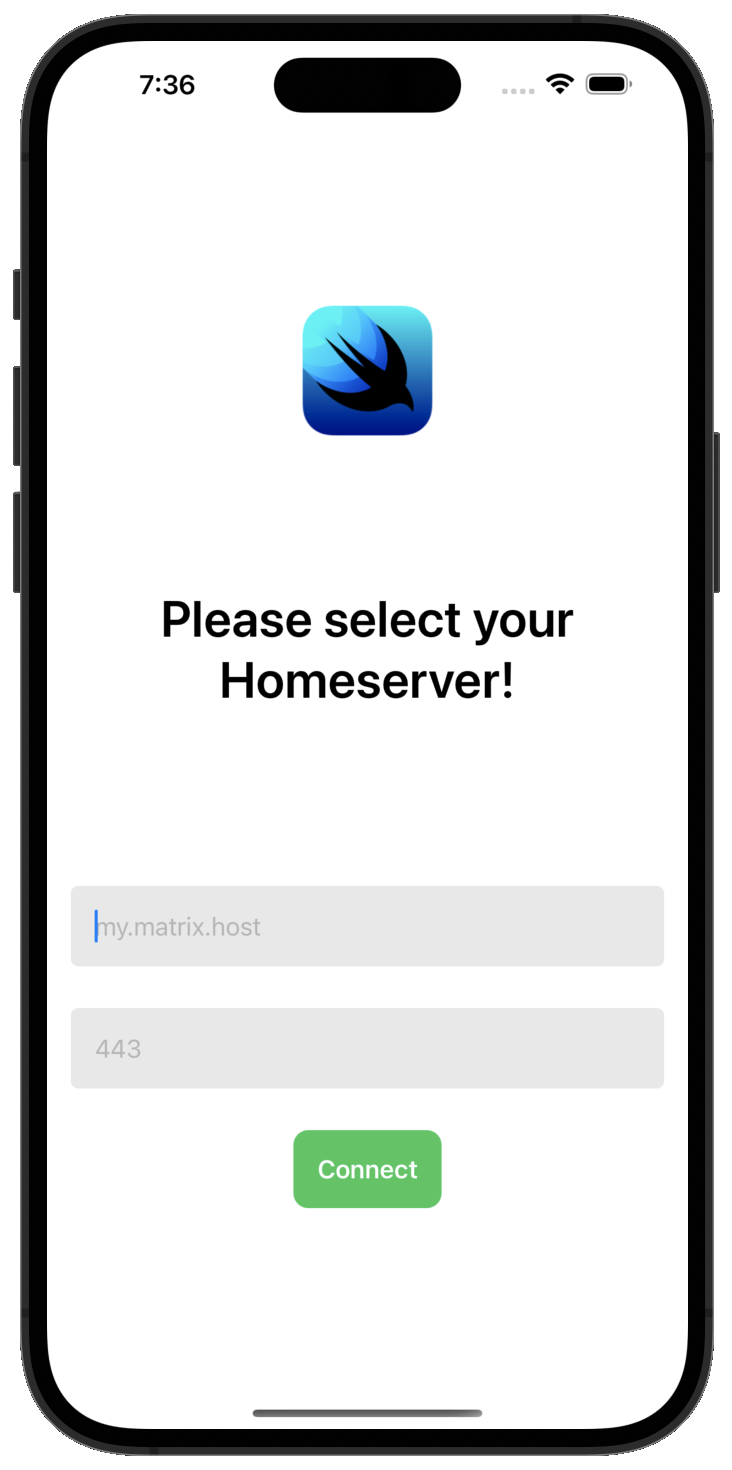
\includegraphics[scale=0.5]{homeserver_white}
        \centering
        \caption{SelectHomeserverView}\label{fig:selecthomeserverview}
    \end{figure}
%    \begin{wrapfigure}{R}{0.5\textwidth}
%        \begin{center}
%            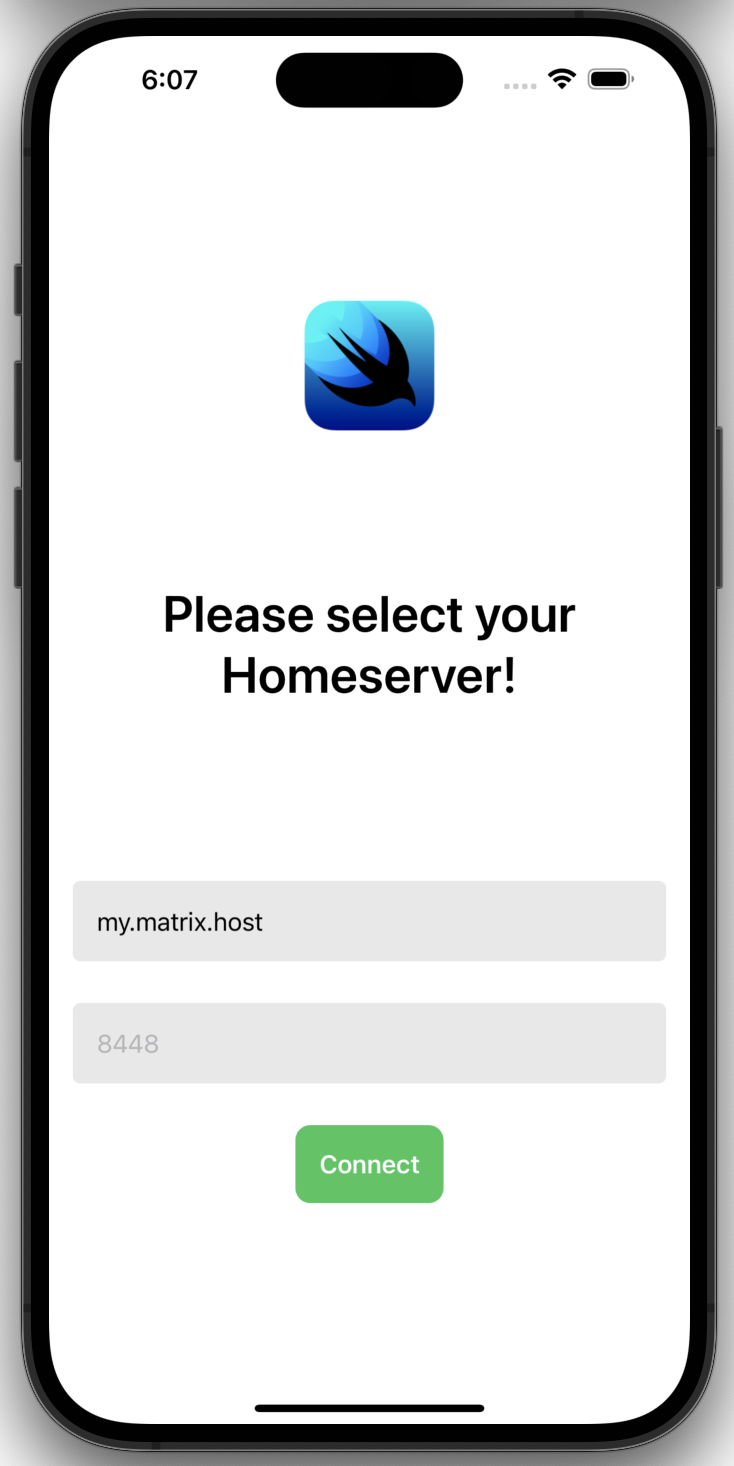
\includegraphics[scale=0.5]{selecthomeserver}
%        \end{center}
%        \caption{SelectHomeserverView}\label{fig:selecthomeserverview}
%    \end{wrapfigure}
    Hat der User einen Homeserver eingetragen und klick auf \("\)Connect\("\) prüft die App zuerst, ob der Homeserver erreichbar ist.
    Hierzu wird eine Abfrage der Versionsnummer an den angegebenen Homeserver gesendet.
    Dies geschieht durch Senden einer GET Anfrage an \texttt{/\_matrix/client/versions} (siehe Abschnitt~\ref{sec:rest}).
    Ist diese Anfrage erfolgreich wird der Homeserver im Model hinterlegt und der User gelangt zur \texttt{LoginView} welche in Abbildung~\ref{fig:loginview} zu sehen ist.
    Falls die Anfrage fehlschlägt, wird dem User eine Fehlermeldung gezeigt.
    \begin{figure}[h]
        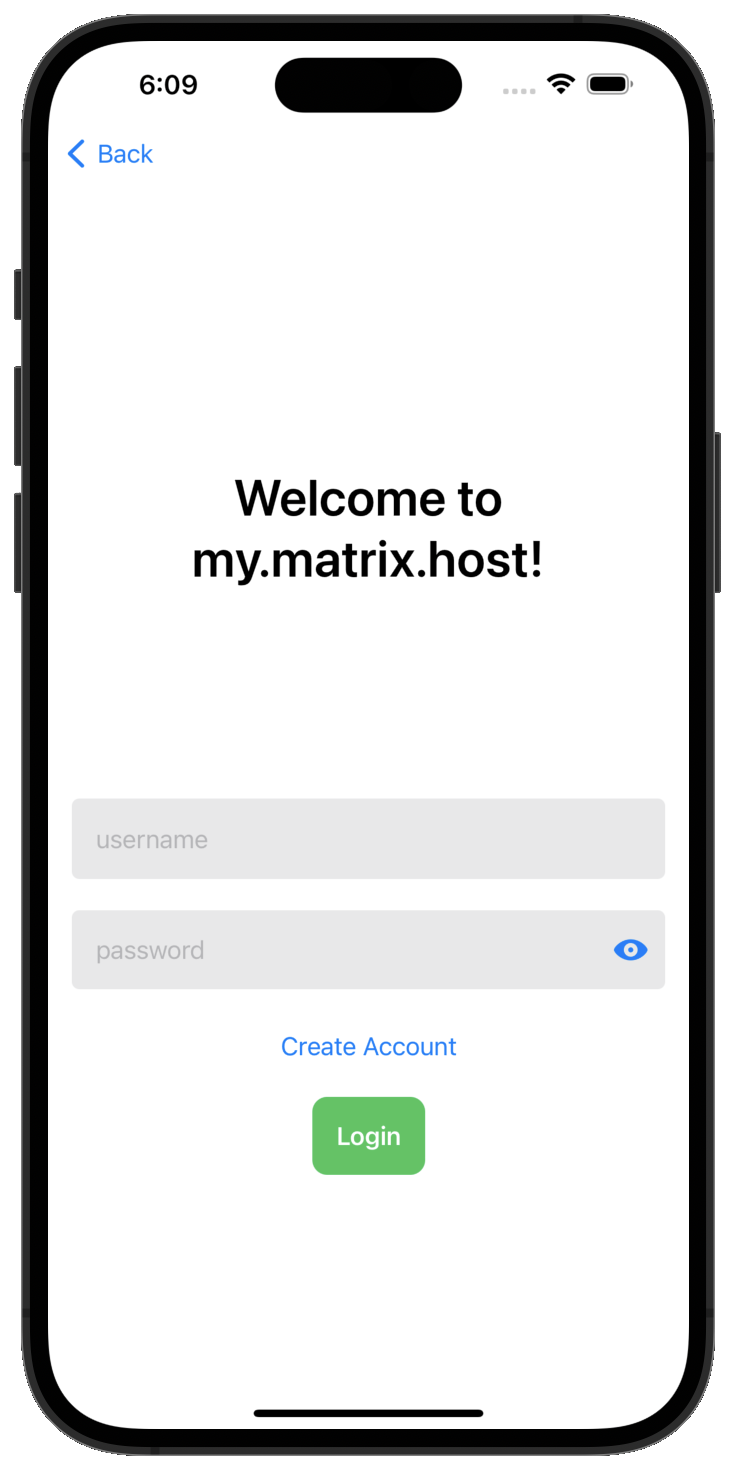
\includegraphics[scale=0.5]{login_white}
        \centering
        \caption{LoginView}\label{fig:loginview}
    \end{figure}
    In dieser View kann der User sich entweder mit seinem bereits existierenden Account anmelden oder einen neuen Account erstellen.
    Für den Fall, dass der User bereits einen Account besitzt, muss er seinen Benutzernamen und sein Passwort in die dafür vorgesehenen Felder eintragen und über den \("\)Login\("\)-Button bestätigen.
    Das Passwortfeld ist hierbei ein \texttt{SecureField} welches die Eingabe versteckt und lediglich mit Punkten darstellt.
    Über das Auge am Rand des Textfeldes kann der User zwischen geschützter Ansicht und Klartext wechseln.

    Hat der User seine Zugangsdaten eingegeben und über den \("\)Login\("\)-Button bestätigt, wird eine Login-Anfrage an den Server gesendet.
    Bei gültigen Zugangsdaten enthält die Antwort des Servers folgende Informationen:
    \begin{description}[leftmargin=!,labelwidth=3cm]
        \item [home\_server] die vollständige Adresse des Homeservers
        \item [access\_token] ein Token der Zugriff auf den Account des Users erlaubt
        \item [user\_id] die vollständige Matrix ID des Users
        \item [device\_id] die vom Server zugewiesene ID für das Gerät
    \end{description}
    Die Information über \texttt{home\_server}, \texttt{user\_id} und \texttt{device\_id} werden in den \texttt{UserDefaults} der App gespeichert , damit diese bei erneutem öffnen der App verfügbar sind..
    Da der \texttt{access\_token} den Zugriff auf Benutzerkonto des Users ermöglicht und deshalb besonders geschützt werden muss, wird dieser mittels eines \texttt{KeychainHelper}\footnote{https://gist.github.com/LeeKahSeng/2452e90a57a5324de367907a36d88a49} in der iCloud Keychain gespeichert.
    Falls die Zugangsdaten nicht korrekt sind, wird dem User erneut eine Fehlermeldung gezeigt.
    Anschließend wird mit diesen Informationen eine Matrix Session gestartet, welche vollen Zugriff auf die auf dem Homeserver gespeicherten Daten erlaubt.
    War das Starten der Session erfolgreich, gelangt der User in die \texttt{RoomsView}.\\
    Für den Fall, dass der User noch keinen Account besitzt, kann dieser über den Button \("\)Create Account\("\) der \texttt{LoginView} zur \texttt{CreateAccountView} gelangen, welche in Abbildung~\ref{fig:createaccountview} dargestellt ist.
    Diese View dient der Accounterstellung und enthält 3 Textfelder für Benutzernamen, Passwort und Registrierungstoken.
    Für das Passwortfeld kann wie schon in der \texttt{LoginView} zwischen versteckter Eingabe und Klartext gewechselt werden.
    \begin{figure}[h]
        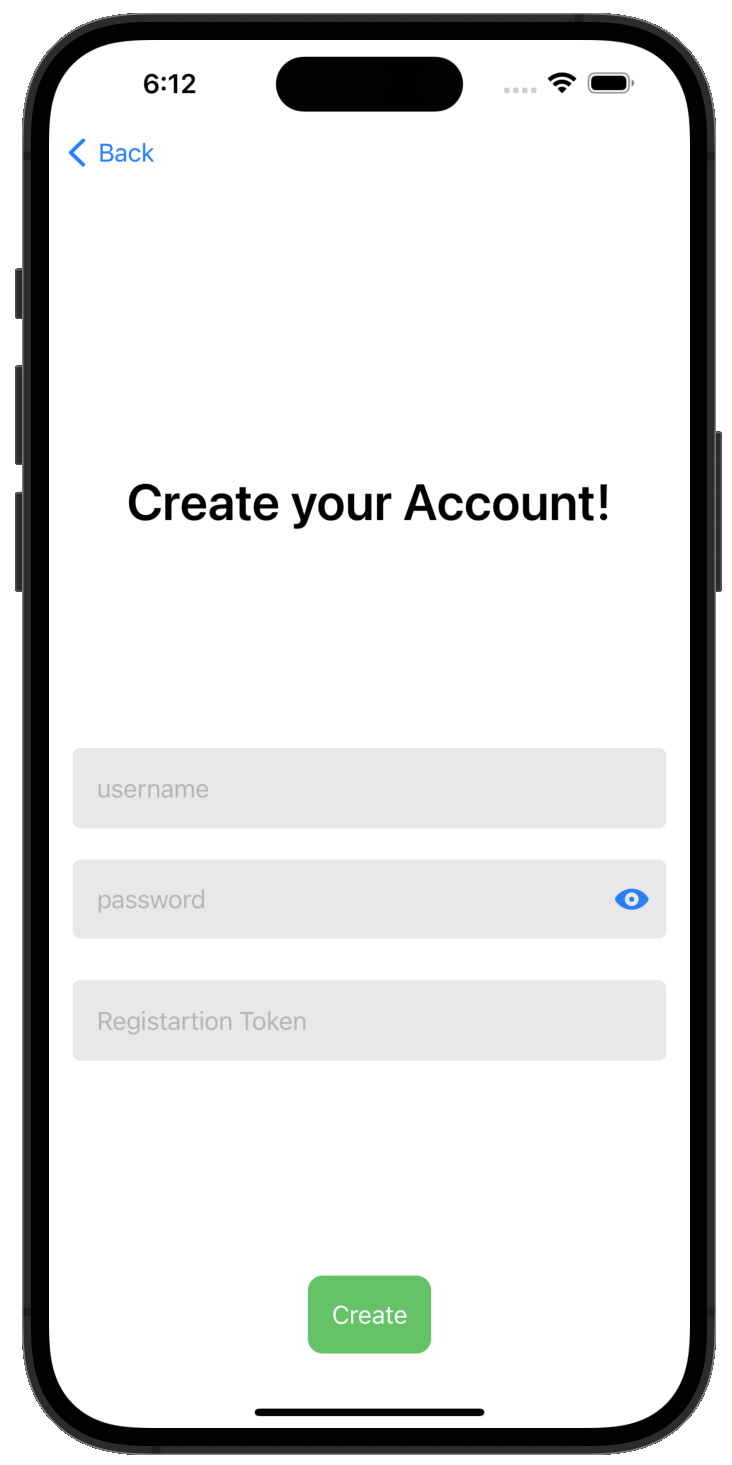
\includegraphics[scale=0.5]{accountcreate_white}
        \centering
        \caption{CreateAccountView}\label{fig:createaccountview}
    \end{figure}
    Der Registrierungstoken kann über die Admin-API\footnote{https://matrix-org.github.io/synapse/latest/usage/administration/admin\_api/} des Servers erstellt werden.
    Hierzu muss eine GET-Anfrage an \texttt{/\_synapse/admin/v1/registration\_tokens/new} gesendet werden.~\cite{synapseregistartiontoken}
    Alternativ kann auch direkt in der Datenbank (in der \texttt{registration\_tokens} Tabelle) des Servers ein Token angelegt werden.

    \newpage
    Es werden folgende Felder bereitgestellt:
    \begin{description}[leftmargin=!,labelwidth=3cm]
        \item [token] Der Token der bei der Erstellung des Accounts angegeben werden muss.
        \item [uses\_allowed] Die maximale Anzahl an Accounts die mit einem Token erstellt werden kann.
        \item [pending] Anzahl laufender Registrierungen.
        Sie gibt an wie viele Benutzer die Authentifizierungsstufe mit dem Token bereits abgeschlossen haben ohne den vollständigen Registrierungsvorgang erfüllt zu haben.
        \item [completed] Anzahl erfolgreich erstellter Accounts mit diesem Token.
        \item [expiry\_time] Er gibt an wie lange der Token gültig ist.
    \end{description}

    Der eigentliche Registrierungsvorgang kann mehrere Authentifizierungsstufen enthalten.
    Bevor der Registrierungsvorgang gestartet wird, wird zuvor mit der vom \texttt{MXRestClient} bereitgestellten Funktion geprüft, ob der Benutzername bereit genutzt wird.
    In dieser Implementation wird der in Abbildung~\ref{fig:accountCreationDiagram} beschriebene Registrierungsvorgang mittels eines Registriersungstokes genutzt.

    \begin{figure}[h]
        \centering
        \begin{sequencediagram}
            \newthread{A}{Client}{}
            \newinst[7]{B}{Server}{}
            \begin{sdblock}{Stage 1}{Receive Session ID}
                \begin{call}{A}{getRegistrationSession()}{B}{\shortstack{
                    return Session ID\\
                    return supported flows}}
                    \postlevel
                \end{call}
            \end{sdblock}
            \begin{sdblock}{Stage 2}{m.login.registration\_token}
                \begin{call}{A}{register()}{B}{}
                \end{call}
            \end{sdblock}
            \begin{sdblock}{Stage 3}{m.login.dummy}
                \begin{call}{A}{register()}{B}{}
                \end{call}
            \end{sdblock}
        \end{sequencediagram}
        \caption{Account erzeugungs Flow}
        \label{fig:accountCreationDiagram}
    \end{figure}

    Der Registrierungsvorgang besteht aus drei Stufen:
    \begin{enumerate}[label={(\arabic*)}]
        \item Im ersten Schritt sendet der Client eine leere Anfrage zum Server, in welcher er um das Starten einer Registrierungssitzung bittet.
    Der Server antwortet daraufhin mit einer Session ID und den vom Homeserver unterstützten Authentifizierungsvorgängen.
    In diesem Beispiel ist der einzige unterstützte Vorgang die Verifizierung über einen Registriersungstoken.
        \item Im nächsten Schritt sendet der Client den zuvor bereitgestellten Registrierungstoken und die vom Server gegebene Session ID in Kombination mit der aktuellen Stufe des Authentifizierungsvorgangs.
        \item Im dritten und letzten Schritt wird nun der \("\)Dummyflow\("\) aufgeführt.
    Dieser Schritt kann nicht fehlschlagen und dient der finalen Erstellung des Accounts.
    Hierbei werden der gewünschte Benutzername und Passwort übergeben.
    \end{enumerate}

    Ist dies geschehen, wurde der Account erfolgreich erstellt.
    Anschließend wird der User ebenfalls auf die \texttt{RoomsView} weitergeleitet.

    \newpage
    \subsection{Raumübersicht}\label{subsec:raumubersicht}

    Die \texttt{RoomsView} ist die Ansicht, die dem User bei jedem Start der App gezeigt wird, sofern er sich bereits in der App angemeldet hat.
    Von dieser Ansicht aus können alle weiteren Views erreicht werden.
    Die in Abbildung~\ref{fig:roomsview} gezeigte View besteht aus einer \texttt{Toolbar} im Kopf der Ansicht, über welche man zur \texttt{ProfileView} und \texttt{SettingsView} gelangt.
    Darunter findet sich die Raumübersicht, welche alle beigetretenen Räume in einer scrollbaren Liste anzeigt.

    \begin{figure}[h]
        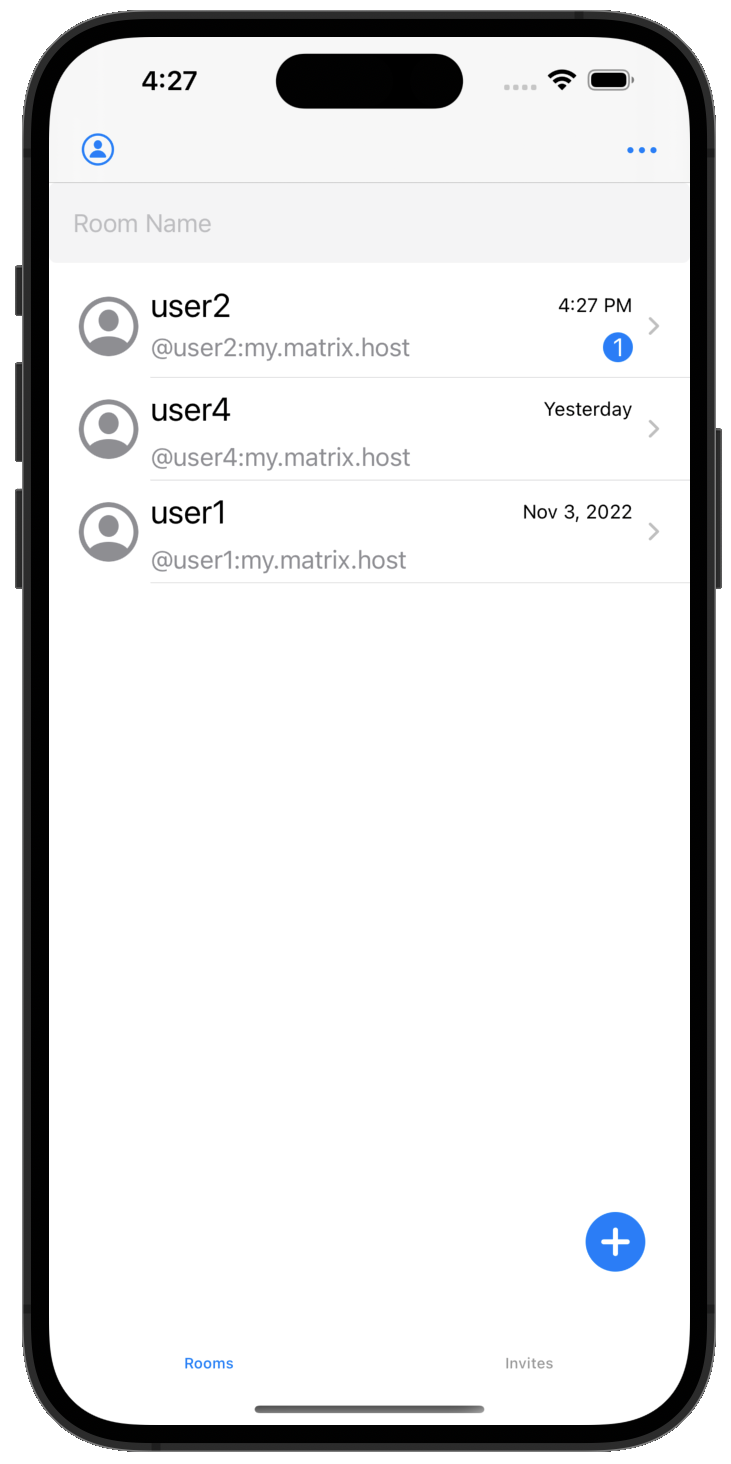
\includegraphics[scale=0.5]{rooms_white}
        \centering
        \caption{RoomsView}\label{fig:roomsview}
    \end{figure}
    Jedes Element der Liste zeigt das Bild des jeweiligen Raumes sowie Anzeigenamen oder Title des jeweiligen Raumes.
    Bei direkten Räumen wird außerdem die Matrix ID des Users angezeigt, da User ihren Anzeigenamen beliebig ändern können.
    Auf das Zeigen einer Vorschau der letzten Nachricht wurde hierbei im Sinne des Datenschutzes bewusst verzichtet.
    Außerdem wird der Zeitpunkt der letzten Nachricht und ein Indikator für die Anzahl ungelesener Nachrichten in einem Raum gezeigt.
    Über das darüberliegende Textfeld kann die Liste gefiltert werden.
    Darüber hinaus wird die Liste nach dem  \texttt{originServerTimestamp} der letzten Nachricht des jeweiligen Raumes sortiert.
    Über den \("\)Plus\("\)-Button gelangt der User zur \texttt{NewRoomView}, über welche ein neuer Raum erstellen werden kann.
    Im Fuß der View befindet sich eine \texttt{TabView} über welche zwischen \texttt{RoomsView} und \texttt{InvitesView} gewechselt werden kann.
    \begin{figure}[h]
        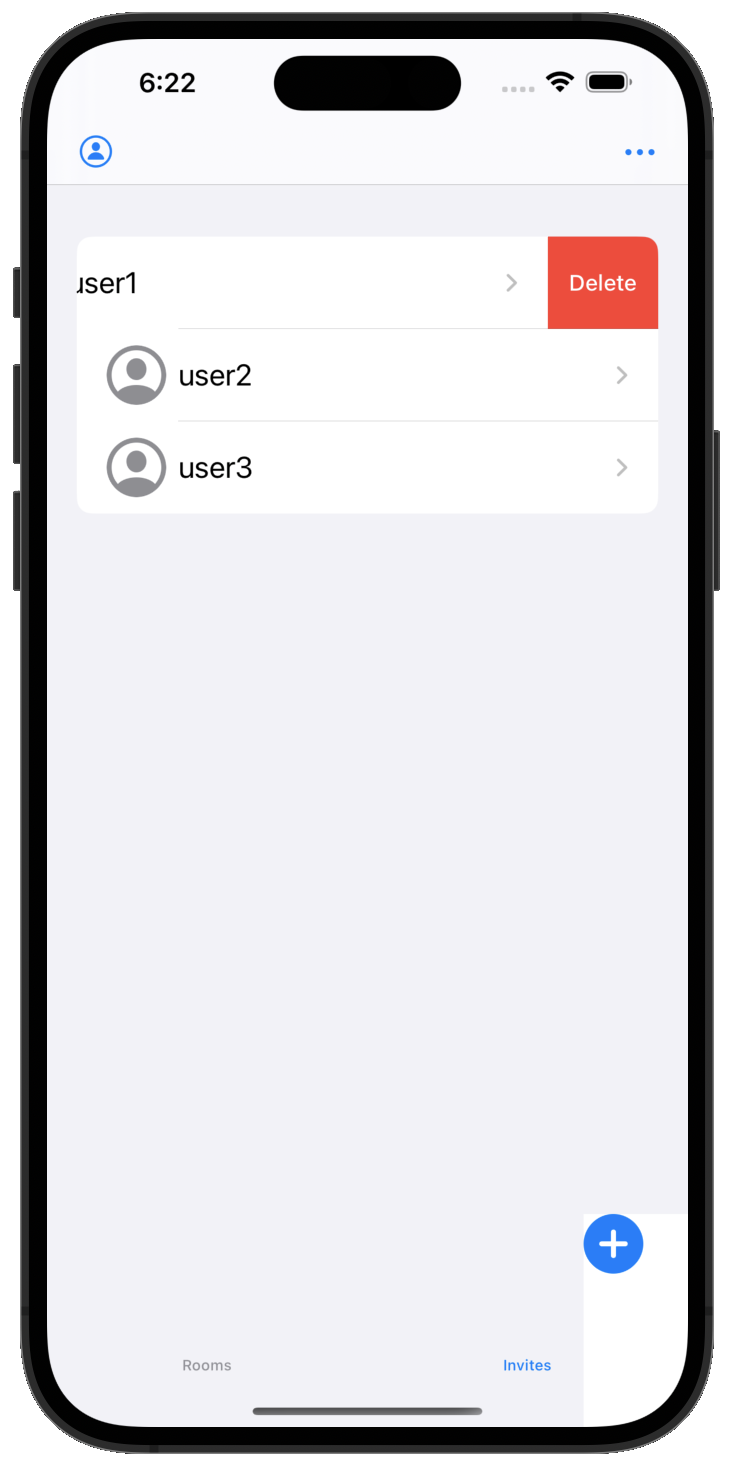
\includegraphics[scale=0.5]{invites_white}
        \centering
        \caption{InvitesView}\label{fig:invitesview}
    \end{figure}
    Die \texttt{InvitesView} welche in Abbildung~\ref{fig:invitesview} zu sehen ist, dient dazu alle offenen Einladungen zu anderen Räumen aufzulisten.
    Diesen kann durch einfaches klicken auf den jeweiligen Raum beigetreten werden.
    Der User gelangt daraufhin direkt in die \texttt{ChatView} des jeweiligen Raumes.
    Durch Wischen der Einladung in Richtung des linken Bildschirmrandes kann die Einladung abgelehnt werden.


    \newpage
    \subsection{Raumerzeugung}\label{subsec:raumerzeugung}
    Hat der User in der \texttt{RoomsView} oder \texttt{InvitesView} auf den Plus-Button geklickt, gelangt er in die \texttt{NewRoomView}.
    Diese View dient dazu, neue Räume zu erstellen und User zu diesen einzuladen.
    Hierzu wird dem User, wie in Abbildung~\ref{fig:newroomview} zu sehen, ein Textfeld gezeigt, über welches er nach anderen Usern suchen kann.
    Für die Suche muss der Anzeigenamen oder die Matrix ID des gewünschten Gesprächsteilnehmers angegeben werden.

    \begin{figure}[h]
        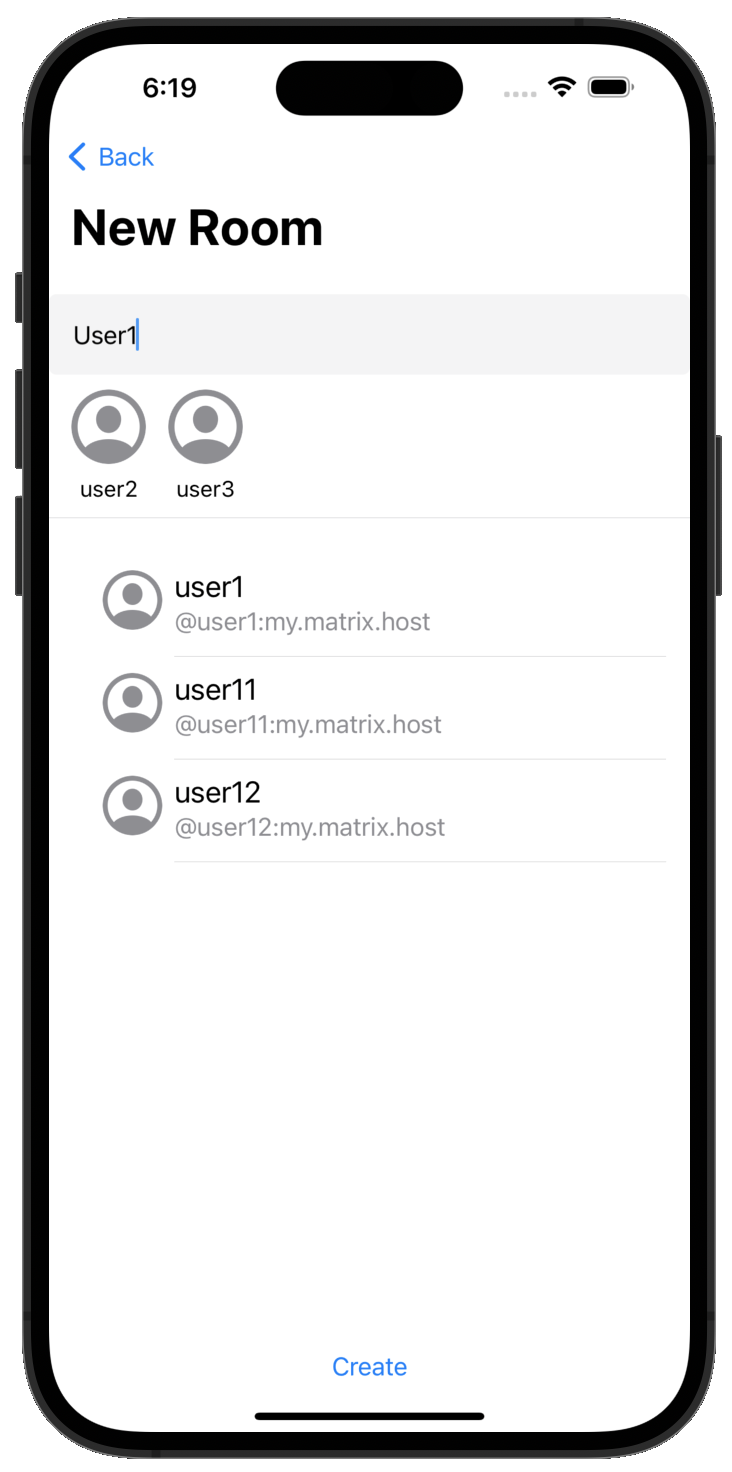
\includegraphics[scale=0.5]{newroom_white}
        \centering
        \caption{NewRoomView}\label{fig:newroomview}
    \end{figure}

    Daraufhin werden in einer scrollbaren Liste bis zu 10 User gezeigt, die dem eingegebenen Suchtext entsprechen.
    Diese Funktion ist nur möglich, falls in der Konfiguration des Homeservers die Suche im Nutzerverzeichnis freigegeben ist.
    Die Konfiguration des Homeservers ist in Abschnitt~\ref{sec:homeserver} genauer beschrieben.
    Ist diese Funktion nicht freigegeben, muss der User die vollständige Matrix ID des gesuchten Gesprächsteilnehmer angeben.
    Hat der User den von ihm gesuchten Gesprächsteilnehmer gefunden, kann er durch Anklicken hinzugefügt werden.
    Der User erscheint dann in der horizontal scrollbaren Liste von Usern.
    Hat der User einen falschen Gesprächsteilnehmer zum Raum hinzugefügt, kann er diesen durch Antippen des Users in der Liste hinzugefügter Gesprächsteilnehmer wieder entfernen.
    Hierbei achtet die App darauf, dass ein Gesprächsteilnehmer nicht doppelt hinzugefügt werden kann.
    Hat der User alle von ihm gewünschten Gesprächsteilnehmer dem Raum hinzugefügt, kann er diesen durch Klicken auf den "Create"-Button erstellen.
    Die App entscheidet automatisch anhand der Anzahl der eingeladenen User, ob ein direkter Raum erstellt werden kann.
    Nach Erstellen des Raumes wird automatisch ein StateEvent von Typ \texttt{.roomEncryption} an den Raum gesendet, welche die anderen Teilnehmer im Raum darüber informiert, dass Nachrichten in diesem Raum verschlüsselt zu senden sind.
    Der vollständige Vorgang zum Verschlüsseln der Nachrichten ist in Abschnitt~\ref{subsec:verschlusselung-der-nachrichten} beschrieben.
    War das Erstellen des Raumes erfolgreich, wird der User in die \texttt{ChatView} des neu angelegten Raumes geleitet.

    \newpage
    \subsection{Chatfenster}
    Die in Abbildung~\ref{fig:chatview} gezeigte \texttt{ChatView} ist eine weitere Kernansicht der App.
    Sie ermöglicht es dem User, Konversationen eines Raumes einzusehen und neue Nachrichten an diesen zu senden.
    Die Abbildung zeigt Beispielnachrichten für alle unterstützten Nachrichtentypen.
    Es können einfache Textnachrichten versendet werden, Fotos welche durch Antippen in einem Vollbild \texttt{ImageViewer} angezeigt werden,
    PDF-Dateien, welche in einem \texttt{PDFViewer} eingesehen werden können, und Videos, welche mittels \texttt{AZVideoPlayer} abgespielt werden können.
    Der Videoplayer unterstützt sowohl das abspielen direkt in der \texttt{ChatView} als auch im Vollbildmodus, sowohl im Hoch- als auch im Querformat.

    \begin{figure}[h]
        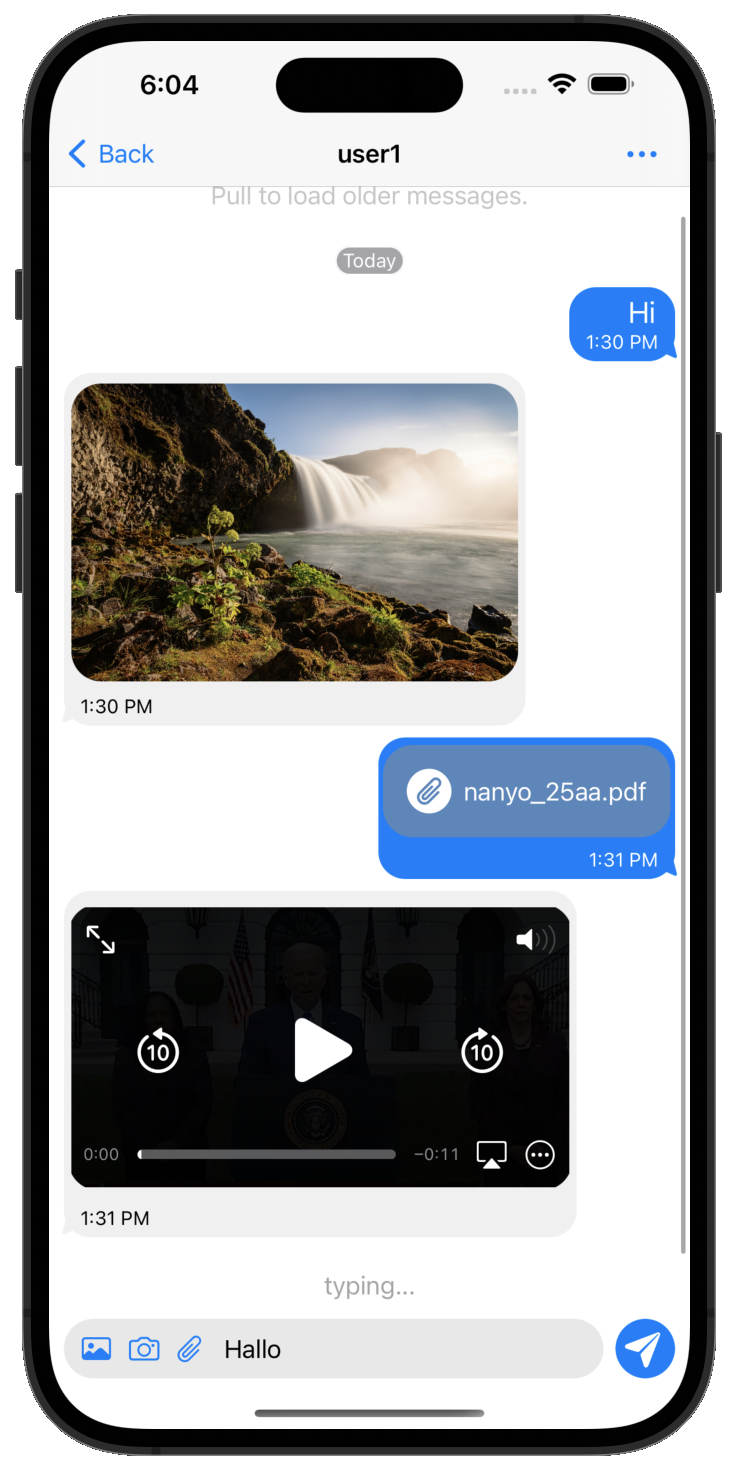
\includegraphics[scale=0.5]{chat_white}
        \centering
        \caption{ChatView}\label{fig:chatview}
    \end{figure}

    Des Weiteren wird dem User ein Typing-Indikator gezeigt, welcher den User darüber informiert, ob der Gesprächspartner (oder in Gruppenräumen welche Gesprächspartner) gerade eine Nachricht schreiben.
    Im Fuß der Ansicht befindet sich das Nachrichtenfenster, über welches Nachrichten verfasst und an der Raum gesendet werden können.
    Durch Klicken des Bild-Icons öffnet sich ein \texttt{ImagePicker}, über welchen sowohl Fotos als auch Videos aus der Galerie gewählt und an den Raum gesendet werden können.
    Das Kamera-Icon öffnet eine Kameraansicht, über welche Fotos und Videos direkt aus der App aufgenommen und versendet werden können.
    Über das Büroklammer-Icon lassen sich Dateien, die auf dem Gerät gespeichert sind, durchsuchen und an den Raum senden.
    Da nur Dateien vom Typ PDF von der App unterstützt werden, wird beim Durchsuchen der Dateien ebenfalls nach PDF gefiltert.
    Im Kopf der Ansicht erkennt man eine Hinweismeldung darauf, dass man das Ende der geladenen Nachrichten erreicht hat und nach unten wischen muss, um weitere Nachrichten zu laden.
    Bei Öffnen der \texttt{ChatView} werden, sofern vorhanden 25 Nachrichten geladen.
    Dies geschieht durch Paginierung des Event-Graphs eines Raumes.
    Bei jedem Laden älterer Nachrichten werden 25 weitere Nachrichten geladen und angezeigt.
    Es muss darauf geachtet werden, dass die Reihenfolge der Nachrichten ordnungsgemäß angezeigt wird.
    Die Lazy-Loading-Methode erlaubt hierbei eine angemessene Performance beim Öffnen des Chats.
    Eine besondere Herausforderung ist die Position der scrollbaren Liste.
    Beim Öffnen der View muss an das Ende der Liste gesprungen werden, da sich dort die neusten Nachrichten befinden.
    Falls eine neue Nachricht eintrifft, während die View geöffnet ist, springt die Liste ebenfalls an das Ende, um dem User die neuste Nachricht anzuzeigen.
    Beim Laden älterer Nachrichten soll jedoch nicht zum Ende gesprungen werden.
    Über die drei Punkte in der oberen rechten Ecke der Ansicht öffnet sich ein Drop-down-Menü, über welches ein Raum verlassen werden kann.
    Außerdem kann eine Übersicht über den aktuellen Raum geöffnet werden, wo Titel, Beschreibung und Bild des Raumes geändert werden können.
    Darüber hinaus zeigt sie einige Informationen über den Raum an, wie die Anzahl der Teilnehmern, den Ersteller des Raumes und ob die Verschlüsselung aktiv ist.

    \newpage
    \subsection{Profile}\label{subsec:profile}
    Die \texttt{ProfileView} welche in Abbildung~\ref{fig:profileview} zu sehen ist, erlaubt dem User seinen Account zu verwalten.
    Durch Klicken auf das Profilbild öffnet sich der \texttt{ImagePicker}, welcher auch schon in der \texttt{ChatView} genutzt wurde, wodurch der User ein neues Profilbild setzen kann.
    Außerdem kann er seinen Anzeigenamen ändern.
    Die Matrix ID bleibt hierbei jedoch gleich.
    Es wird dem User die Möglichkeit geboten, sein Passwort zu ändern.
    Hierfür öffnet sich nach Klicken des Buttons eine Infobox, welche den User um Eingabe seines alten und seines neuen Passworts bittet.
    Falls das alte Passwort korrekt eingegeben wurde, wird das neue Passwort gesetzt.\\

    \begin{figure}[h]
        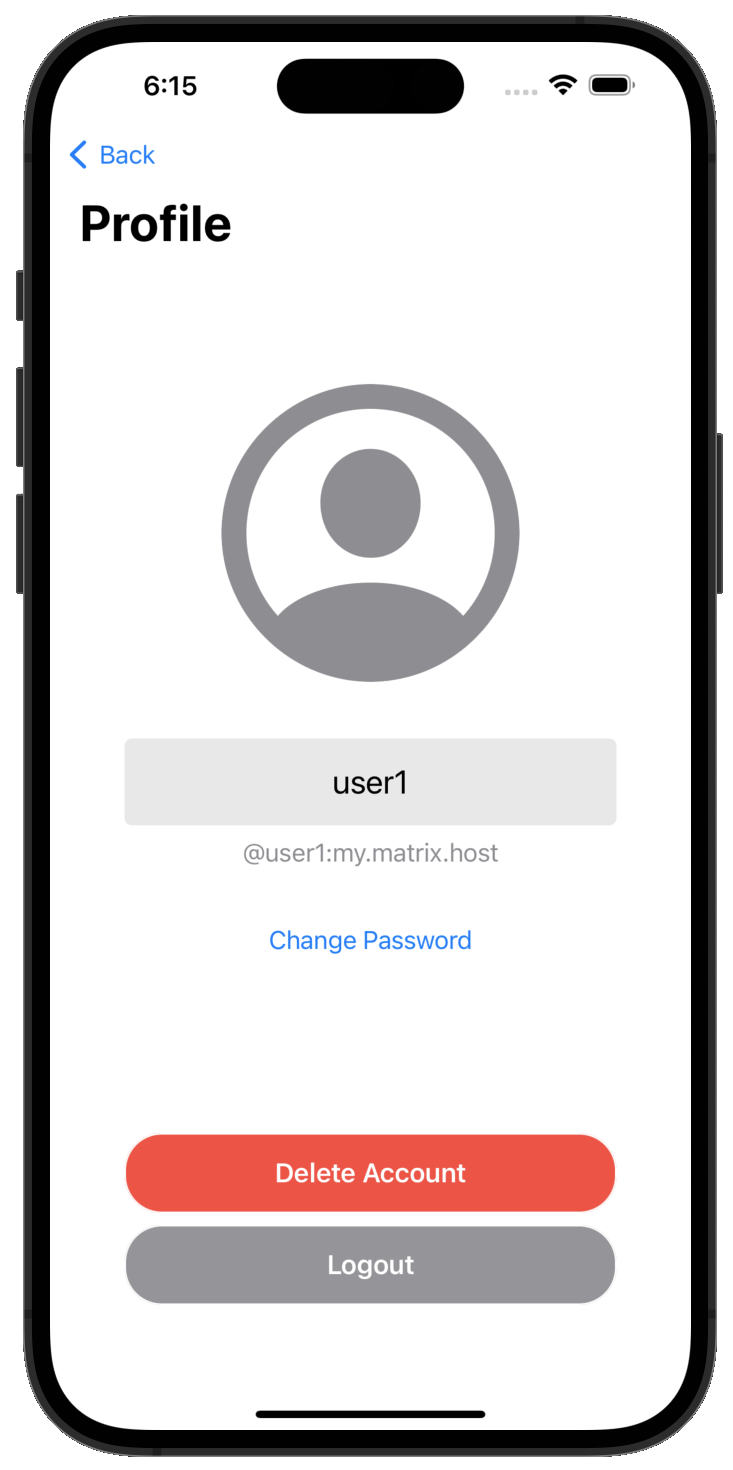
\includegraphics[scale=0.5]{profile_white}
        \centering
        \caption{ProfileView}\label{fig:profileview}
    \end{figure}
    Im unteren Teil der Ansicht befinden sich zwei Buttons.
    Der \("\)Logout\("\)-Button ermöglicht es dem User, sich von einem Gerät abzumelden.
    Hierbei werden alle zuvor gespeicherten Daten in der Keychain und den \texttt{UserDefaults} gelöscht und der User gelangt wieder in die \texttt{SelectHomeserverView}.
    Der \("\)Delete Account\("\)-Button erlaubt es dem User, seinen Account dauerhaft zu deaktivieren.
    Nach Klicken des Buttons wird der User aufgefordert, dies mit seinem Passwort zu bestätigen.
    Es ist zu beachten, dass beim Löschen des Accounts aktuell keine zuvor versendeten Nachrichten oder Daten gelöscht werden.

    \subsection{Verschlüsselung der Nachrichten}\label{subsec:verschlusselung-der-nachrichten}
    Zur Verschlüsselung der Nachrichten sind mehrere Schritte notwendig.
    Zuerst muss die Verschlüsselung in der Sitzung aktiviert werden.
    Dies geschieht durchstarten und aktivieren des Kryptomoduls der SDK.
    Dabei werden die im Abschnitt~\ref{subsec:verwendete-schlussel} aufgeführten Schlüssel erstellt und mit dem Server synchronisiert.
    Zusätzlich muss beim Erstellen eines Raumes zuallererst ein Encryption Event gesendet werden, welches die anderen Teilnehmer eines Raums darüber informiert, dass die Kommunikation in einem Raum verschlüsselt zu erfolgen hat.
    Hierbei muss der für die Verschlüsslung der Nachricht verwendete Algorithmus angegeben werden.
    Zurzeit wird nur die \texttt{m.megolm.v1.aes-sha2} Verschlüsselung unterstützt.
    Falls nun eine Nachricht über die Sitzung an den erstellten Raum gesendet wird, wird diese beim Senden automatisch von der SDK verschlüsselt.
    Beim Empfangen von Nachrichten wird das Event ebenfalls automatisch entschlüsselt.
    Bei Fotos, Videos und Dateien ist zu beachten, dass das Event lediglich einen Pfad zum Ablageort der gesendeten Datei auf dem Server enthält.
    Diese Dateien müssen separat heruntergeladen werden.
    Da die Dateien nach dem Herunterladen noch immer verschlüsselt sind, müssen diese anschließend mit Hilfe der SDK entschlüsselt werden.
    Anhand der Notwendigkeit des Entschlüsselns der Dateien kann bestätigt werden, dass die Verschlüsslung aktiv ist.
    Zusätzlich kann auf dem Homeserver unter \texttt{/data/media\_store} geprüfte werden, dass die Dateien verschlüsselt auf dem Server abgelegt werden.

    \subsection{Benachrichtigungen}\label{subsec:benachrichtigungen}
    Damit der User nicht in regelmäßigen Abständen überprüfen muss, ob er neue Nachrichten erhalten hat, muss diesem beim Eintreffen einer neuen Nachricht eine Benachrichtigung gesendet werden.
    Hierzu wird beim Starten der Anwendung ein \texttt{EventListener} konfiguriert, welcher an die Matrix Session übergeben wird.
    Dieser \texttt{EventListener} filtert neu eintreffende Events nach ihrem \texttt{type} und sendet eine entsprechende Benachrichtigung über das \texttt{UNUserNotificationCenter} an den User.
    Hierbei wird darauf geachtet, ob der User den Raum, in dem die Nachricht versendet wurde, auf dem Bildschirm geöffnet hat.
    In diesem Fall wird keine Benachrichtigung gesendet.
    Der \texttt{EventListener} wird ebenfalls genutzt, um dem User bei Eintreffen eines Typing-Events einen Typing-Indikator zu zeigen.\\
    Es ist zu beachten, dass dies nur funktioniert, solange die App aktiv läuft.
    Um Benachrichtigungen zu erhalten, wenn die App geschlossen ist, muss die Anwendung über den Apple-Push-Notification-Service (ASPN) registriert und mit dem Push-Gateway des Matrix Homeservers verbunden werden.
    Da Push-Notifications vom Simulator nicht unterstützt werden, konnte dieser Teil nicht getestet werden und wird deshalb nicht weiter behandelt.

    \newpage
    \section{Homeserver}\label{sec:homeserver}
    Der Homeserver bildet die unterliegende Infrastruktur der Plattform.
    Hierfür wird das vom Matrix Team bereitgestellte Synapse Docker Image verwendet.
    Diese wird in einem Docker Container auf dem Server betrieben.
    Bevor der Container gestartet werden kann, werden einige Konfigurationsdateien benötigt, welche über folgenden Befehl generiert werden können:
    \begin{lstlisting}[language=bash,label={lst:synapse-generate}]
docker run -it --rm -v /path/on/host/machine/:/data -e SYNAPSE_SERVER_NAME=my.matrix.host -e SYNAPSE_REPORT_STATS=yes matrixdotorg/synapse:latest generate
    \end{lstlisting}
    Um später einfacher Änderungen an der Konfiguration des Homeservers vornehmen zu können, wird das \texttt{/data} Directory im Host gemountet.
    Des Weiteren muss der Name des Homeservers über \texttt{SYNAPSE\_SERVER\_NAME} definiert werden.
    Dieser wird später für die Identifikation des Homeservers genutzt.
    Nach Ausführen des Befehls werden 3 Dateien generiert:
    \begin{description}[leftmargin=!,labelwidth=4cm]
        \item [homeserver.yaml] Konfigurationsdatei des Homeservers. Hier können alle Funktionalitäten des Homeservers konfiguriert werden.
        \item [my.matrix.host.log.config] Konfigurationsdatei des Loggers. Hier kann das Format für Log-Messages definiert werden.
        \item [my.matrix.host.signing.key] Key zur Authentifizierung bei anderen Homeservern.
    \end{description}

    Der \texttt{my.matrix.host.signing.key} wird für diese Implementation nicht benötigt, da der Homeserver nicht an das Matrix-Netzwerk angeschlossen wird.
    Bevor der Server gestartet wird, müssen noch einige Konfigurationen angepasst werden:
    \begin{enumerate}[label={(\arabic*)}]
        \item Standardmäßig wird nur ein Listener auf Port 8008 für ungeschützte Verbindungen über HTTP konfiguriert.
            Um die App mit dem Homeserver verbinden zu können, muss ein zusätzlicher HTTPS Listener auf Port 443 konfiguriert werden.
        \begin{lstlisting}[language=yaml,label={lst:listener}]
listeners:
  - port: 443
    type: http
    tls: true
    resources:
          - names: [client]
            \end{lstlisting}
        \item Für den zusätzlichen Listener über HTTPS muss ein SSL Zertifikat erstellt und in der Konfiguration hinterlegt werden. Während der Entwicklung wurde hierfür ein selbst signiertes Zertifikat mittels Open SSL generiert.
            \begin{lstlisting}[language=yaml,label={lst:ssl-certificate}]
tls_certificate_path: "/data/certs/cert.pem"
tls_private_key_path: "data/certs/key.pem"
            \end{lstlisting}
        \item Da während der Entwicklung ein selbst signiertes Zertifikat verwendet wurde, muss zusätzlich die Zertifikat-Verifikation ausgeschaltet werden.
            \begin{lstlisting}[language=yaml,label={lst:disable-cert}]
federation_verify_certificates: false
            \end{lstlisting}
        \item Da der Server nicht mit dem Matrix-Netzwerk verbunden wird, muss die Schlüsselverifizierung über den Matrix Root Server deaktiviert werden.
            \begin{lstlisting}[language=yaml,label={lst:disable-key-verification}]
trusted_key_servers:
  - server_name: "matrix.org"
    accept_keys_insecurely: true
            \end{lstlisting}
        \item Um das in Abschnitt~\ref{subsec:raumerzeugung} beschriebene durchsuchen des Nutzerverzeichnisses zu ermöglichen, muss dies hier erlaubt werden.
            \begin{lstlisting}[language=yaml,label={lst:user-directory}]
user_directory:
  enabled: true
  search_all_users: true
            \end{lstlisting}
        \item Zusätzlich können Regeln aktiviert werden, die beim Erstellen eines Accounts prüfen, ob das Passwort den gewünschten Richtlinien entspricht.
                Hier kann definiert werden, welche Arten von Zeichen im Passwort enthalten sein müssen und wie lang das Passwort mindestens sein muss.
            \begin{lstlisting}[language=yaml,label={lst:password-policy}]
password_config:
   enabled: true
   localdb_enabled: true
   pepper: "EVEN_MORE_SECRET"

   policy:
      enabled: true
      minimum_length: 8
      require_digit: true
      require_symbol: true
      require_lowercase: true
      require_uppercase: true
            \end{lstlisting}
        \item Da die Registrierung nur mit einem Registrierungstoken möglich sein soll, muss dies ebenfalls angegeben werden.
        \begin{lstlisting}[language=yaml,label={lst:enable-registration}]
enable_registration: true
registration_requires_token: true
        \end{lstlisting}
        \item Als weiter Absicherung, dass auch alle Räume verschlüsselt sind, werden Raume standardmäßig verschlüsselt.
    \begin{lstlisting}[language=yaml,label={lst:enable-encryption}]
encryption_enabled_by_default_for_room_type: all
    \end{lstlisting}
    \end{enumerate}

    Nachdem alle Konfigurationen getätigt wurden, kann der Homeserver gestartet werden.
    Es ist darauf zu achten, dass alle benötigten Ports des Containers über den Host freigegeben werden.

    \begin{lstlisting}[language=bash,label={lst:synapse-start}]
docker run -d --name synapse -v /path/on/host/machine/:/data -p 8008:8008 -p 443:443 matrixdotorg/synapse:latest
    \end{lstlisting}

    Nach dem Start des Containers ist der Homeserver einsatzbereit und Clients können eine Verbindung aufnehmen.
    Es wird außerdem eine Datenbank angelegt.
    Für die Implementation wird die standardmäßig konfigurierte SQLite Datenbank verwendet.
    Hier werden alle für den Betrieb des Homeservers benötigten Tabellen angelegt.
    Zudem wird ein \texttt{media\_store} Ordner angelegt, welcher alle versendeten Dateien der Nutzer enthält.

    \newpage
    \chapter{Evaluation}\label{ch:evaluation}
    In diesem Kapitel werden die in Abschnitt~\ref{sec:anforderungen} definierten Anforderungen auf ihre Implementation geprüft.
    Hierbei werden die mit \("\)Won't" priorisierten Anforderungen nicht beachtet.

    \newpage
    \section{Must-Anforderungen}\label{sec:must-anforderungen}
    \begin{table}[h]
        \centering
        \begin{tabular}{p{0.57\textwidth}|p{0.37\textwidth}}
            Anforderung & Status\\
            \cline{1-2}
            Der User muss über die App einen Account auf der Plattform anlegen können.
            &  \textbf{Erfüllt} \\
            \cline{1-2}
            Der User muss sich mit seinem Account in der App einloggen können. &  \textbf{Erfüllt} \\
            \cline{1-2}
            Der User muss sein Passwort ändern können. & \textbf{Erfüllt}  \\
            \cline{1-2}
            Dem User muss alle von ihm beigetretenen Räume sehen können. &  \textbf{Erfüllt} \\
            \cline{1-2}
            Dem User muss neue Räume erstellen können. & \textbf{Erfüllt} \\
            \cline{1-2}
            Der User muss zu neuen Räumen eingeladen werden können. & \textbf{Erfüllt} \\
            \cline{1-2}
            Der User muss alle Nachrichten die in einem Raum gesendet wurden, einsehen können. & \textbf{Erfüllt} \\
            \cline{1-2}
            Nachrichten Inhalte müssen verschlüsselt, separat vom allgemeinen Speicherbereich des Endgeräts abgelegt werden. & \textbf{Erfüllt} (keine lokale Speicherung implementiert) \\
            \cline{1-2}
            Der User muss Nachrichten in einem Raum senden können. & \textbf{Erfüllt} \\
            \cline{1-2}
            Nachrichten zwischen Usern müssen End-to-End verschlüsselt sein. & \textbf{Erfüllt} \\
            \cline{1-2}
            Der Usern muss Nachrichten löschen können. & \textbf{Nicht Erfüllt} \\
            \cline{1-2}
            Der User muss einen Raum verlassen können. & \textbf{Erfüllt} \\
            \cline{1-2}
            Der User muss seinen Account deaktivieren können. & \textbf{Erfüllt} (kein automatisches Löschen der Daten erfolgt)\\
            \cline{1-2}
            Die App darf keinen Zugriff auf das Adressbuch des Endgerätes haben. & \textbf{Erfüllt}
        \end{tabular}
        \caption{Übersicht über erfüllte Must-Anforderungen}
        \label{tab:erfüllte-must-anforderungen}
    \end{table}

    \newpage
    \section{Should-Anforderungen}\label{sec:should-anforderungen}
    \begin{table}[h]
        \centering
        \begin{tabular}{p{0.57\textwidth}|p{0.37\textwidth}}
            Anforderung & Status\\
            \cline{1-2}
            Beim Erstellen des Accounts soll eine zusätzliche Authentifizierungsmethode verwendet werden, um böswilliges Erstellen von Accounts zu verhindern.
            &  \textbf{Erfüllt} (mittels Registrierungstoken)\\
            \cline{1-2}
            Der User soll sich nur einmal einloggen müssen. &  \textbf{Erfüllt} \\
            \cline{1-2}
            Der User soll sich ausloggen können. & \textbf{Erfüllt}  \\
            \cline{1-2}
            Der Benutzer soll die Möglichkeit haben, sein Profilbild und seinen Anzeigenamen anzupassen. &  \textbf{Erfüllt} \\
            \cline{1-2}
            Der vollständige Chat-Verlauf soll nur bei Bedarf geladen werden. & \textbf{Erfüllt} (Lazy-Loading)\\
            \cline{1-2}
            Die App soll neben Textnachrichten auch andere Nachrichtentypen wie Fotos, Videos oder Audiodateien unterstützen. & \textbf{Teilweise Erfüllt} (unterstützt Foto, Video und PDF) \\
            \cline{1-2}
            Die App soll den User über den Erhalt einer neuen Nachricht informieren. & \textbf{Erfüllt} \\
            \cline{1-2}
            Der User muss Nachrichten in einem Raum senden können. & \textbf{Erfüllt} \\
            \cline{1-2}
            Die Übersicht der beigetretenen Räume soll nach letzter Aktivität sortiert werden. & \textbf{Erfüllt}
        \end{tabular}
        \caption{Übersicht über erfüllte Should-Anforderungen}
        \label{tab:erfüllte-should-anforderungen}
    \end{table}

    \newpage
    \section{Could-Anforderungen}\label{sec:could-anforderungen}
    \begin{table}[h]
        \centering
        \begin{tabular}{p{0.57\textwidth}|p{0.37\textwidth}}
            Anforderung & Status\\
            \cline{1-2}
            Die Liste der beigetretenen Räume kann gefiltert werden. &  \textbf{Erfüllt} \\
            \cline{1-2}
            Dem Erstellen eines Raumes kann dem User eine Liste von Usern vorgeschlagen werden, welche dem gesuchten Namen entsprechen. & \textbf{Erfüllt}  \\
            \cline{1-2}
            Dem User kann ein Typing-Indikator gezeigt werden. &  \textbf{Erfüllt} \\
            \cline{1-2}
            Die App kann auch mit anderen Homeservern verbunden werden. & \textbf{Teilweise Erfüllt} (Accounterstellung nicht möglich)\\
            \cline{1-2}
            Der User kann den Inhalt einer Textnachricht in die Zwischenablage kopieren. & \textbf{Nicht Erfüllt} \\
            \cline{1-2}
            Der User kann eine Nachricht weiterleiten. & \textbf{Nicht Erfüllt}  \\
            \cline{1-2}
            Der User kann Dateien, welche in einem Raum verschickt wurden, herunterladen. & \textbf{Nicht Erfüllt}  \\
            \cline{1-2}
            Die App kann im Querformat mode genutzt werden. & \textbf{Teilweise Erfüllt}
        \end{tabular}
        \caption{Übersicht über erfüllte Could-Anforderungen}
        \label{tab:erfüllte-could-anforderungen}
    \end{table}


    \chapter{Fazit}\label{ch:fazit}
    Die Plattform erfüllt die grundlegenden Funktionen einer Messaging-App.
    Sie bietet die Möglichkeit einen Account anzulegen, zu verwalten und wieder zu löschen.
    Sie erlaubt das Erstellen, Beitreten und Löschen von Räumen sowohl in Direkt- als auch in Gruppenräumen.
    Das Senden und Empfangen von Nachrichten geschieht in Echtzeit und mit End-to-End-Verschlüsselung, sodass der Betreiber der Plattform keinerlei Zugriff auf die Daten der User hat.
    Dabei unterstützt die Plattform die gängigsten Nachrichtentypen und sorgt dafür, dass keine personenbezogenen Daten auf dem Gerät gespeichert sind.\\
    Betrachtet man jedoch die Anforderungen, welche von der DSGVO an eine Messaging-App im medizinischen Bereich gestellt werden, muss man feststellen, dass eine Vielzahl weiterer Funktionen implementiert werden müssen, bevor sie als DSGVO-konform eingestuft werden kann und somit zum Einsatz in der Praxis zugelassen wird.
    Das Matrix-Protokoll unterstützt den Großteil der notwendigen Implementierungen, um DSGVO-konform zu werden.
    Die einzige nicht unterstützte Funktionalität, die während der Implementation entdeckt wurde, ist das Löschen von Nachrichten bzw. Inhalten auf dem Server.
    Hierzu wird vom Protokoll zurzeit noch keine Möglichkeit bereitgestellt und somit muss ein eigenes System zum Löschen der Daten entwickelt werden.
    Es ist jedoch möglich, über ein \texttt{m.room.redaction} Event den Inhalt einer Nachricht unkenntlich zu machen.\\
    Zwar sind alle Nachrichten und Daten, die in einem Raum versendet wurden, verschlüsselt und vor unbefugtem Zugriff geschützt, allerdings ist es dem Betreiber der Plattform möglich, die Mitgliedschaften von Nutzern zu Räumen einzusehen.
    Somit könnte abgeleitet werden, welche Personen welche Ärzte besuchen.
    Ob dies zulässig ist, müsste separat untersucht werden.

%    Zwar wurde während der Implementierung darauf geachtet, dass jegliche Daten zwischen Arzt und Patient verschlüsselt und vor unbefugtem Zugriff geschützt sind, jedoch müsste die genaue Rechtslage zum Einsatz der Plattform genauer untersucht werden.
%    Das Userinterface der App erfüllt zwar die gesetzten Ansprüche jedoch lässt das Design noch deutlich Platz für Verbesserungen.
%    Alle im Kapitel~\ref{sec:anforderungen} als 'Must' definierten Funktionen sind implementiert.
%    Ebenfalls wurden alle Anforderungen aus der

    \chapter{Ausblick}\label{ch:ausblick}
    Der nächste Schritt in der Entwicklung der Plattform sollte es sein, die Cross-Signing-Funktion der End-to-End-Verschlüsselung zu unterstützen.
    Hierfür muss ein geeignetes Key-Management-System implementiert werden, welches es ermöglicht ein Gerät von einem anderen zu verifizieren und die Schlüssel, die zur Verschlüsselung der Nachrichten verwendet wurden zu validieren.
    Darüber hinaus sollte ein Prozess implementiert werden, der es ermöglicht, auch ohne Zugriff auf eines der anderen Geräte die verwendeten Schlüssel wiederherzustellen.
    Somit könnte beispielsweise bei Verlust oder bei Beschädigung des Gerätes trotzdem noch auf bestehende Chat-Verläufe zugegriffen werden.
    Mittels des Recovery Services des Kryptomoduls kann ein Backup der Session Keys auf der Server angelegt werden, welches über einen Recovery Key oder eine Passphrase geschützt werden kann.
    Von diesem Backup können dann bei Bedarf alle gespeicherten Keys wiederhergestellt werden.
    Die Dokumentation hierfür ist noch in der Erstellung~\cite{advancede2e}, was die Implementation zum aktuellen Zeitpunkt deutlich erschwert.\\
    Es sollte ein System zum lokalen Speicher der Daten entwickelt werden, welches es möglich macht, die Anwendung auch ohne Verbindung zum Internet einsehen zu können.
    Hierbei muss darauf geachtet werden, die Daten verschlüsselt und separat vom allgemeinen Speicherbereich des Endgeräts abzulegen.
    Außerdem werden dadurch Ladezeiten reduziert und der Datentransfer zwischen Server und Anwendung minimiert.\\
    Des Weiteren kann die Plattform um zusätzliche Nachrichtentypen erweitert werden.
    Es könnte beispielsweise das Aufnehmen und Versenden von Audiodateien hinzugefügt werden.
    Zusätzlich kann der Datei-Message-Typ um weiter Dateitypen erweitert werden.

%    Außerdem könnte ein zusätzlicher Layer implementiert werden, welcher es ermöglicht Informationen über beigetretene Räume und deren jeweilige Konversationen geschützt auf dem Gerät zu speichern.
%    Somit hat der User auch ohne bestehende Verbindung zum Internet, Zugriff auf seine Konversationen und mögliche geteilter Daten.
%    Ferner sollten zusätzliche Dateitypen für Nachrichten unterstützt werden um es
%
%    Des weiteren könnte untersucht werden ob der Synapse Server in der LAge ist den Registrierungstoken über einen SMTP Server direkt an den User zu schicken nach vorheriger angabe einer emailadresse.

%\include{source/content/Test}

%Das Fazit
%\include{source/content/Fazit}
%Einbinden des Abbildungsverzeichnisses

    \backmatter
%Liste der Tabellen
    \listoftables
%Einbinden des Tabellenverzeichnisses
    \listoffigures
%Einbinden des Sourcecodeverzeichnisses
%\lstlistoflistings

% Quellenverzeichnis
    \bibliographystyle{IEEEtran}
    \bibliography{Bachelorarbeit}

% Anhang
    \appendix

\end{document}



%
% EOF
%